%####################################################################
%############ BEGIN PREAMBLE ########################################
%####################################################################
\documentclass[12pt]{report}

\edef\restoreparindent{\parindent=\the\parindent\relax}

%Packages-------------------------------------
\usepackage{parskip}
\usepackage{amsmath}
\usepackage{amsfonts}
\usepackage{amssymb}
\usepackage{amsthm}
\usepackage{graphics}
\usepackage{graphicx}
\usepackage{subfigure}
\usepackage{relsize}
\usepackage{tabularx}
\usepackage{multirow}
\usepackage[nopostdot,style=list,nonumberlist,toc]{glossaries}
%\usepackage{hyperref}
\usepackage{xurl}
\usepackage[nottoc]{tocbibind}
\usepackage{caption}
\usepackage{float}
\usepackage{setspace}

%\usepackage{xtocnic}

\usepackage[localise=on]{xepersian}

\settextfont[Scale=1]{XB Zar}
%\setdigitfont[Scale=1]{XB Zar}
\setlatintextfont[Scale=1]{Times New Roman}
\restoreparindent

%Layout---------------------------------------

%\usepackage[top=2cm, bottom=2cm, left=2cm, right=2cm]{geometry}

%Commands-------------------------------------
\setcounter{tocdepth}{3}
\setcounter{secnumdepth}{3}
\renewcommand{\arraystretch}{1.25}

%Theorems-------------------------------------
\newtheorem{thm}{قضیه}[chapter]
\newtheorem{cor}[thm]{نتیجه}
\newtheorem{defn}[thm]{تعریف}
\newtheorem{prop}[thm]{گزاره}
\newtheorem{lmm}[thm]{لم}
\newtheorem{conj}[thm]{حدس}
\newtheorem{exm}[thm]{مثال}
\newtheorem{rem}[thm]{تذکر}
\newtheorem{note}[thm]{یادداشت}
\newtheorem{alg}[thm]{الگوریتم}


%Glossaries-----------------------------------
\makeglossaries
\loadglsentries{glossaries}

%Folder of Figures----------------------------
\graphicspath{{./figures/}}
%####################################################################
%########### END PREAMBLE ###########################################
%####################################################################


%####################################################################
%########### BEGIN DOCUMENT #########################################
%####################################################################
\begin{document}
	\thispagestyle{empty}
	
\includegraphics[width=1\linewidth]{besmela}
	\newpage
	
	%Title page ----------------------------------
	
	\begin{figure}
		\centering
		
\includegraphics[height=2.5cm]{ut.png}
	\end{figure}
	
	\begin{center}
		دانشکدگان علوم
		\\
		دانشکده ریاضی، آمار و علوم کامپیوتر
	\end{center}
	
	\begin{center}
		%%%%%%%%%%%%%
	\end{center}
	
	\begin{center}
		\huge{مدل‌سازی سازوکارهای مسئله‌ی انقیاد در شبکه‌های عصبی ضربه‌ای}
	\end{center}
	
	\begin{center}
		%%%
	\end{center}
	
	\begin{center}
		نگارنده
	\end{center}
	\begin{center}
		\textbf{
			امیر اصلان اصلانی
			\\[30pt]
		}
	\end{center}
	
	\begin{center}
		اساتید راهنما
	\end{center}
	\begin{center}
		\textbf{
			محمد گنج‌ تابش 
			\\[5pt]
			عباس نوذری دالینی
		}
	\end{center}
	
	\vspace{3cm}
	\begin{center}
		پایان‌نامه برای دریافت درجه‌ی کارشناسی ارشد
		\\
		در رشته علوم کامپیوتر
	\end{center}
	
	\begin{center}
		بهمن ۱۴۰۱
	\end{center}
	
	\pagestyle{empty}
	\pagenumbering{}
	\newpage







\thispagestyle{empty}
\begin{center}
	
\includegraphics[width=0.2\linewidth]{logo.png}
	\\
	\vspace*{0.6cm}
	دانشگاه تهران\\
	\vspace*{0.6cm}
	اداره کل تحصیلات تکمیلی\\
	\vspace*{3cm}
	{{\huge \bf \centerline{تعهد نامه اصالت اثر}}}
\end{center}
\vspace{0.3cm}

اينجانب  امیر اصلان اصلانی متعهد مي شوم كه مطالب مندرج در اين پايان نامه حاصل كار پژوهشي اينجانب است و به دستاوردهاي پژوهشي ديگران كه در اين پژوهش از آنها استفاده شده است، مطابق مقررات ارجاع و در فهرست منابع و مآخذ ذكر گرديده است. اين پايان نامه قبلاً براي احراز هيچ مدرک هم سطح يا بالاتر ارائه نشده است. در صورت اثبات تخلف (در هر زمان) مدرك تحصيلي صادر شده توسط دانشگاه از اعتبار ساقط خواهد شد.

\vskip .5cm\noindent
کلیه حقوق مادی و معنوی این اثر متعلق به  دانشکده‌ی ریاضی، آمار و علوم کامپیوتر  دانشگاه تهران است.
\vspace{1cm}








	
	\newpage
	%\pagestyle{headings}
	%\setcounter{page}{1}
	%\pagenumbering{roman}
	\pagestyle{plain}
	\setcounter{page}{1}
	\pagenumbering{harfi}
	
	%Abstract page-------------------------------
	
	\chapter*{}
	\section*{چکیده}
	مسئله‌ی انقیاد یکی از مسائل مهم در علوم اعصاب، علوم شناختی و فلسفه‌ی ذهن است که درباره‌ی چگونگی یکپارچه شدن درک موجود زنده از محیط با استفاده از مفاهیم جزئی تشکیل‌شده در مغز است. اهمیت این مسئله در درک عملکرد‌‌های شناختی انسان است که خود بخشی از مراحل مورد نیاز برای طراحی سیستم‌هایی است که قادر به پردازش عملکرد‌های شناختی مشابه انسان هستند. تحقیقات نشان‌دهنده‌ی نقش بسیار پررنگ ستون‌های قشری مغز، که ساختار‌هایی در نوقشر هستند، در عملکرد‌های شناختی موجودات زنده است. در این پژوهش تلاش شده تا با مدل‌سازی ستون‌های قشری و روابط بین آن‌ها با استفاده از شبکه‌های عصبی ضربه‌ای،فرآیند تشکیل انقیاد در مغز شبیه‌سازی شود.  آزمایش‌ها و بررسی‌های صورت گرفته روی مدل پیشنهادی، به درستی شکل‌گیری انقیاد را نشان می‌دهند. این موضوع نشان‌دهنده‌ی این است که احتمالا ستون‌های قشری، به عنوان ساختار‌هایی ثابت و قابل تکرار، بالقوه ساختار‌های مناسبی برای استفاده در مدل‌سازی‌ها هستند و امکان شکل‌‌گرفتن پردازش‌های شناختی را در مدل‌های محاسباتی افزایش می‌دهند. 
	
	\section*{}
	\textbf{کلمات کلیدی:}\quad ستون قشری، مسئله‌ی انقیاد، شبکه‌ی عصبی ضربه‌ای، مدل‌سازی.
	
	%Dedication page-----------------------------
	
	%\chapter*{تقدیم به}
	%\section*{تقدیم به}
	
	%Acknowledgement page------------------------
	
	%\chapter*{سپاسگزاری}
	%\begin{center}
	%    content...
	%\end{center}
	%
	%%copyright + declaration page
	%\chapter*{اصالت اثر}
	%\section*{اصالت اثر}
	% هیچ قسمت از این پایان‌نامه، پیش از این در هیج موسسه تحصیلات عالی برای دریافت درجه تحصیلی استفاده نشده است. همچنین، هیچ قسمت از این پایان‌نامه برگردان فارسی تمامی یا قسمتی از یک اثر دیگر علمی (مانند مقاله، پایان‌نامه، و غیره) به زبانی دیگر نمی‌باشد. ارائه این پایان‌نامه توسط نگارنده به معاونت آموزشی (معاونت پژوهشی و تحصیلات تکمیلی برای ارشد و دکتری) به منزله تعهد نگارنده به اصالت متن و محتوای ارائه‌شده بر اساس یک کار پژوهشی در مدت تحصیل در دانشگاه تهران می باشد. در صورت اثبات خلاف این امر، مدرک تحصیلی اخذ شده توسط این پایان‌نامه از دانشگاه تهران، معتبر نمی باشد.
	%
	%\chapter*{حق مالکیت معنوی}
	%\section*{حق مالکیت معنوی}
	%حق مالکیت معنوی این اثر متعلق به دانشگاه تهران می باشد. استفاده از مطالب این پایان‌نامه در فعالیت‌های تحقیقاتی با ذکر منبع بلامانع می‌باشد. در صورت استفاده تجاری، مانند چاپ این پایان‌نامه، هماهنگی لازم و اجازه کتبی از دانشگاه و نگارنده پایان‌نامه الزامی می‌باشد.
	%
	
	%-------------------------
	%\pagestyle{plain}
	%\setcounter{page}{1}
	%\pagenumbering{harfi}
	%-------------------------
	\onehalfspacing
	%Preface--------------------------------------
	
	\chapter*{پیشگفتار }
	برای مدت زمان بسیاری چگونگی کارکرد مغز انسان یکی از  سؤالات بشر بوده و در دهه‌های اخیر، دانش ما از ساختار مغز با پیشرفت فناوری بسیار افزایش یافته‌‌است؛ اما همچنان چگونگی رخدادن بسیاری از عملکرد‌های شناختی در موجودات زنده، از اصلی‌ترین پرسش‌های پژوهشگران هستند. افزایش دانش ما از ساختار مغز با پیدایش سیستم‌های محاسبه‌گر و پس از آن با افزایش قدرت محاسباتی آن‌ها همراه بوده که موجب پیشرفت‌های بسیار چشم‌گیری در حوزه‌ی هوش مصنوعی شده‌است. کنجکاوی بشر در چگونگی عملکرد مغز انسان از یک سو و پیشرفت‌های هوش مصنوعی از سوی دیگر باعث شده تا بسیاری از پژوهشگران با تلاش برای مدل‌سازی فعالیت‌های مغزی به سمت تولید سیستم‌های هوشمند با عملکرد‌های شناختی مشابه انسان گام بردارند. در این میان علوم ‌اعصاب محاسباتی به عنوان یک حوزه‌ی بین رشته‌ای، که از طرفی با علوم اعصاب در ارتباط است و از طرف دیگر با علم کامپیوتر، در سال‌های اخیر پیشرفت‌های بسیاری داشته‌است که موجب شده تا بسیاری از محققان به پژوهش در این حوزه روی‌آورند.
	
	یکی از موضوعات اساسی که چگونگی رخدادن آن در موجودات زنده همچنان به صورت واضح مشخص نشده‌است، مسئله‌ی انقیاد است. موجودات زنده محیط خود را از طریق ورودی‌های عصبی همچون بینایی، شنوایی و لامسه احساس می‌کنند و تک‌تک اجزای اطلاعات دریافت‌شده به صورت مجزا و تفکیک‌شده در مغز شکل می‌گیرند؛ ولی  موجود زنده به یک درک یکپارچه از مفاهیم اطراف خود می‌رسد. برای مثال در مغز فردی که تصویر یک مربع مشکی که با رنگ قرمز پر شده‌‌است را می‌بیند، به صورت مجزا مفهوم چهار خط مشکی و رنگ قرمز شکل می‌گیرد ولی در پردازش‌های شناختی  این مفاهیم جدا از هم به صورت یک مفهوم واحد تجمیع می‌شوند و یک مربع با رنگ قرمز را در ذهن فرد تداعی می‌کنند.
	
	پدیده‌ی انقیاد به عنوان یکی از مهم‌ترین ویژگی‌های شناختی انسان مورد توجه بسیاری از پژوهشگران قرار گرفته‌است و در عصر امروز که هوش مصنوعی و به خصوص شبکه‌های عصبی مصنوعی با سرعت بسیاری در حال پیشرفت هستند، عدم امکان رخدادن انقیاد در آن‌ها به عنوان یکی از محدودیت‌های اصلی بیان می‌شود و به همین دلیل تلاش‌های بسیاری برای پیاده‌سازی سازوکار‌هایی برای وارد کردن انقیاد به شبکه‌های عصبی مصنوعی در حال انجام است. شبکه‌های عصبی مصنوعی ضربه‌ای به عنوان نسل سوم شبکه‌های عصبی مصنوعی و یک مدل زیست‌توجیه‌پذیر، یک ابزار بسیار مناسب برای طراحی مدلی است که انقیاد در آن قابل مشاهده باشد. به همین منظور، در این مطالعه مدلی زیست‌توجیه‌پذیر با استفاده از شبکه‌های عصبی ضربه‌ای و با الهام از ساختار‌هایی به نام ستون‌های قشری در مغز پیاده‌سازی شده‌است که در تلاش است تا سازوکار انقیاد را به صورت محاسباتی مدل‌سازی کند.
	
	این پایان‌نامه در پنج فصل به صورت زیر تنظیم شده‌است:
	
در فصل اول، برخی از مفاهیم اولیه‌ی مرتبط با سیستم عصبی انسان، مسئله‌ی انقیاد و شبکه‌های عصبی ضربه‌ای را به صورت مختصر مرور خواهیم کرد.

در فصل دوم با بیان مسئله‌ی کلی مورد نظر و مشکلات حال حاضر در آن موضوع، به طرح مسئله‌ای که قصد پاسخ به آن را داریم خواهیم پرداخت.

در فصل سوم به برخی از دیگر تلاش‌های صورت‌گرفته در راستای مسئله‌ی مطرح‌شده، ویژگی‌ها، نواقص و نقاط قوت آن‌ها خواهیم پرداخت.

در فصل چهارم به تشریح مدل ارائه‌شده و چگونگی عملکرد آن خواهیم پرداخت. همچنین در ادامه، به بررسی نتایج حاصل‌شده و کسب نتیجه‌ی مدنظر، که مشاهده‌ی انقیاد در مدل است، خواهیم پرداخت.

در فصل پنجم، که فصل نهایی این پایان‌نامه است، یک نگاه کلی به مدل‌های پیشین و مقایسه‌ی ویژگی‌های آن‌ها با مدل ارائه‌شده خواهیم داشت و پس از آن نیز با توجه به نتایج حاصل‌شده از مطالعه، نتیجه‌ی گرفته‌شده را مطرح خواهیم کرد. همچنین در انتهای این فصل به فعالیت‌های دیگری که در ادامه‌ی این مطالعه می‌توان انجام داد، خواهیم پرداخت. 
	
	
	
	%Table of Contents----------------------------
	
	\tableofcontents
	%\listoffigures
	
	%#######################################################
	%#######################################################
	%#######################################################
	%#######################################################
	
	%Chapter One----------------------------------
	
	\chapter{مفاهیم اولیه}
	\label{ch:Defs}
	%*********************
	\pagestyle{plain}
	\setcounter{page}{1}
	\pagenumbering{arabic}
	%*********************
	
	در این فصل به تعریف برخی از مفاهیم اولیه خواهیم پرداخت. بدین منظور از سیستم عصبی انسان شروع خواهیم کرد و به مواردی چون ساختار اعصاب، تغییرات آن‌ها در مرور زمان، سازوکار پاداش و برخی تقسیم‌بندی‌ها درباره‌ی نواحی مغز خواهیم پرداخت. در ادامه اشاره‌ای به روش‌‌های رایج مدل‌سازی در موضوع شبیه‌سازی شبکه‌های عصبی خواهد شد و در نهایت با توضیحاتی در باب مسئله‌ی \gls{binding} فصل را خاتمه خواهیم داد.
	
	%=========================
	\section{سیستم عصبی انسان}
	
	به صورت کلی \gls{nervousSystem} انسان به دو بخش کلی تقسیم می‌شود: \gls{cns}\LTRfootnote{Central Nervous System (CNS)}
	و \gls{pns}\LTRfootnote{Peripheral Nervous System (PNS)}.
	در اینجا موضوعی که بیشتر مورد بحث می‌باشد، سیستم عصبی مرکزی، به‌ویژه مغز است. \gls{cortex} انسان به طور تخمینی از ۲۱ الی ۲۶ میلیارد \gls{neuron} تشکیل شده‌است~\cite{Pelvig2008-vh}
	که در بخش‌های بعدی با جزئیات بیشتری به ساختار و ارتباطات میان آن‌ها خواهیم پرداخت.
	
	
	اطلاعات مختلف که از ارگان‌های حسی انسان (\gls{pns}) ارسال شده‌اند در \gls{brain} تجمیع می‌شوند. سپس مغز این تصمیم را که ارگان‌های بدن چه اعمالی را باید انجام دهند، اتخاذ می‌کند. مغز داده‌های خام را برای استخراج اطلاعاتی درباره‌ی محیط، پردازش می‌کند و سپس این اطلاعات را با نیاز‌های فعلی انسان و اطلاعاتی که در حافظه از شرایط گذشته دارد ترکیب می‌کند تا در نهایت بر اساس نتایج حاصل‌شده، یک الگوی حرکتی را تولید ‌کند. این پردازش اطلاعات نیازمند تعاملاتی پیچیده میان بخش‌های مختلف سیستم عصبی است 
	\cite{carew2000}.
	
	\subsection{ساختار نورون‌ها}
	
	نورون‌ها سلول‌هایی هستند که وظیفه‌ی اصلی پردازش را در سیستم عصبی موجودات زنده بر عهده دارند. به صورت خاص، نورون‌ها سیگنال‌هایی را دریافت، پردازش و منتقل می‌کنند. نورون‌ها از نظر شکل، اندازه و خواص الکتروشیمیایی بسیار متنوع هستند. آن‌ها از چند بخش اصلی، به شرح زیر تشکیل شده‌اند: (شکل \ref{fig:neuron})
	\begin{itemize}
		\item \gls{soma}\LTRfootnote{Soma} یا جسم سلولی که شامل هسته‌ی سلول\LTRfootnote{Nucleus} است و فعالیت‌های حیاتی سلول داخل آن اتفاق می‌افتد.
		\item \gls{dendrite}\LTRfootnote{Dendrite} که یک جسم شاخه‌مانند است و نقش دریافت سیگنال‌های ارسال‌شده توسط نورون‌های دیگر را که توسط آکسون‌های آن‌ها منتقل شده‌است، بر عهده دارد.
		\item \gls{axon}\LTRfootnote{Axon} که جسمی شاخه‌مانند است، سیگنال‌های ارسالی از نورون را به \gls{dendrite}‌های نورون‌های دیگر منتقل می‌کند. سرعت انتقال پیام‌‌ در آکسون متغیر است و بستگی به میزان \gls{myelin}\LTRfootnote{Myelin} در اطراف آن دارد.
	\end{itemize}
	
	\begin{figure}[]
		\centering
		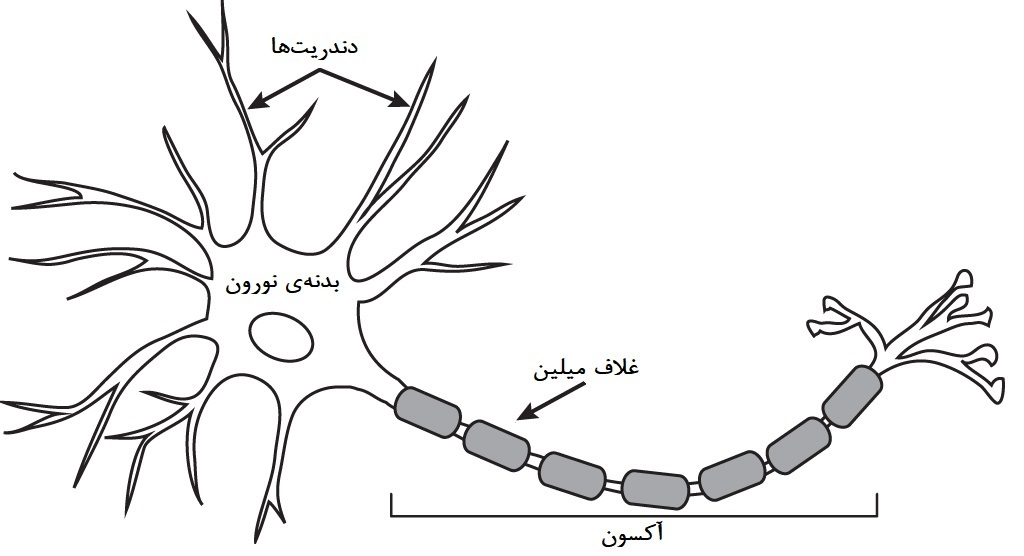
\includegraphics[width=0.7\linewidth]{neuron.jpg}
		\caption[NS]{
			اجزای تشکیل دهنده‌ی نورون\footnotemark.
		}
		\label{fig:neuron}
	\end{figure}
	
	% اینا همشون برعکس شدن (لاتین‌ها و اعداد. نسخه‌ی ۴ هست ولی برای درست نشون داده شدن برعکس نوشته شده)
	\RTLfootnotetext{
		خلق‌شده توسط
		Henley Casey 
		تحت مجوز
		BY-NC-SA CC
		نسخه ۰.۴.
	}
	
	
	بدنه‌ی نورون از یک لایه‌ی عایق تشکیل شده‌است که سبب ایجاد اختلاف پتانسیل بین داخل و خارج نورون می‌شود. همچنین مجموعه‌ای از \gls{ionchannels}\LTRfootnote{Ion Channels} نیز وجود دارند که نورون از طریق آن‌ها یون‌هایی را با محیط بیرون تبادل می‌کند و این تبادلات موجب تغییر در میزان اختلاف پتانسیل نورون می‌شود. زمانی که اختلاف پتانسیل یک نورون از یک آستانه فراتر رود، مجموعه‌ای از این کانال‌ها باز شده و موجب افزایش بسیار سریع اختلاف پتانسیل و سپس کاهش مجدد آن به میزان طبیعی می‌شود. به این پدیده، شلیک یا \gls{spike}\LTRfootnote{Spike} می‌گوییم. در زمان رخدادن پدیده‌ی \gls{spike}، همراه با افزایش ناگهانی اختلاف پتانسیل در نورون، این اختلاف پتانسیل از طریق آکسون‌ها منتقل‌شده و در سیناپس‌ها \gls{neurotransmitters}\LTRfootnote{Neurotransmitter} را آزاد می‌کند  که در نتیجه باعث افزایش یا کاهش اختلاف پتانسیل در دندریت‌های مجاور این سیناپس‌ها می‌شود. در این فرآیند، نورونی که منشأ اختلاف پتانسیل منتقل‌شده بوده‌است را \gls{pre}‌\LTRfootnote{Pre-synaptic Neuron} و نورونی را که این اختلاف پتانسیل به آن منتقل شده، \gls{post}‌\LTRfootnote{Post-synaptic Neuron} می‌نامیم.
	
	نورون‌ها را از جهت‌های گوناگونی، همچون عملکرد و ساختار فیزیکی، میتوان دسته‌بندی کرد~\cite{NARAYANAN2016183}. آن‌ها از نظر عملکرد به دو دسته‌ی کلی تقسیم می‌شوند؛ دسته‌ی اول نورون‌های تحریکی\LTRfootnote{Excitatory} هستند که در سیناپس‌هایشان انتقال‌دهنده‌های عصبی تحریکی مثل \gls{Glutamate}\LTRfootnote{Glutamate} آزاد می‌شود و اختلاف پتانسیل را در \gls{post} افزایش می‌دهند. دسته‌ی دوم نورون‌های مهاری هستند که در سیناپس‌هایشان انتقال‌دهنده‌های عصبی مهاری مثل \gls{GABA}\LTRfootnote{GABA} آزاد می‌شود و اختلاف پتانسیل را در \gls{post} کاهش می‌دهند~\cite{Purves2001-ns}.
	
	همچنین، می‌توان از جهت ساختار فیزیکی نورون‌ها را به سه دسته‌ی کلی تقسیم کرد:
\gls{unipolar}\LTRfootnote{Unipolar Neurons}،
\gls{bipolar}\LTRfootnote{Bipolar Neurons}
و نورون‌های چند‌قطبی\LTRfootnote{Multipolar Neurons} \cite{brainitel01736978}. 
	نورون‌های تک‌قطبی از یک شاخه‌ی کوتاه تشکیل شده‌اند که خود به دو شاخه تقسیم می‌شود که در دو راستای مخالف‌هم حرکت می‌کنند. نورون‌های دو‌قطبی دو شاخه دارند که در خلاف جهت یکدیگر هستند. نورون‌های چندقطبی، نورونی است که یک آکسون و چندین دندریت دارد و امکان تجمیع اطلاعات چندین نورون دیگر را دارد. ساختار این سه دسته از نورون‌ها در شکل \ref{fig:neurontypes} مشخص شده است.
	
	\begin{figure}[]
		\centering
		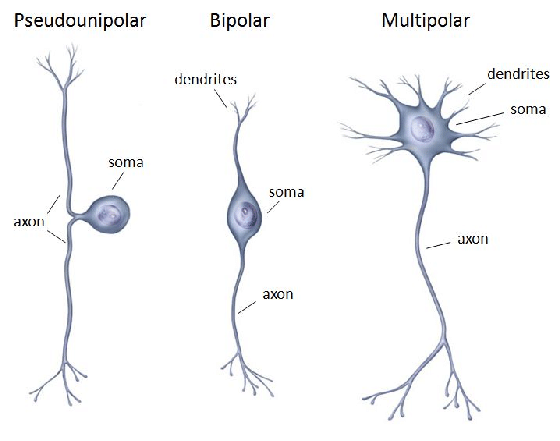
\includegraphics[width=0.7\linewidth]{neurontypes.png}
		\caption[NS]{
			تقسیم‌بندی نورون‌ها از جهت ساختار فیزیکی آن‌ها.
		}
		\label{fig:neurontypes}
	\end{figure}
	
	\subsection{\gls{neocortex} و \gls{cc}}
	\gls{neocortex} یک قشر مغزی شش‌لایه در پستانداران است که وظیفه‌ی عملکرد‌های سطح بالایی همچون شناخت، حرکت، بینایی و گفتار را برعهده دارد
	\cite{Lui2011}. شماره‌گذاری لایه‌های \gls{neocortex} به ترتیب از بیرونی‌ترین لایه شماره ۱ تا درونی‌‌ترین لایه، شماره‌ی ۶ می‌باشد.
	همچنین \gls{neocortex} شامل نورون‌های تحریکی و مهاری با نسبت تقریبی ۸۰٪ به ۲۰٪ است
	\cite{noback2005human}.
	
	ساختار \gls{neocortex} علاوه براین‌که شامل شش لایه‌ی افقی می‌باشد، شامل مجموعه‌ای از سازه‌های عمودی به نام \gls{cc} است که سطح مقطع بسیار کوچکی در ابعاد نیم میلی‌متر دارند و \gls{neocortex} از کنار‌ هم قرار‌گرفتن این ستون‌ها شکل می‌گیرد
	\cite{Horton2005}.
	به صورت کلی، این ستون‌های قشری از نظر ارتباط بین لایه‌ها الگوی‌های تکرار‌شونده‌ای دارند که در تمام بخش‌های \gls{neocortex} مشابه یکدیگر هستند. \gls{ccc}\LTRfootnote{Canonical Cortical Circuit}، که توسط داگلاس و مارتین 
	\cite{Douglas2004}
	بیان شده‌است، ارتباط بین بخش‌های مختلف داخلی و بین ستون‌های قشری را نشان می‌دهد
	(شکل \ref{fig:cc-doganmart}).
	
	\begin{figure}[]
		\centering
		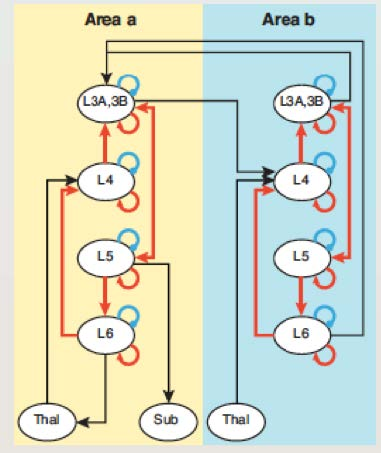
\includegraphics[width=0.6\linewidth]{cc-con.jpg}
		\caption[NS]{
			مدار قشری استاندارد که توسط داگلاس و مارتین بیان شده‌است
			\cite{Douglas2004}.
			در این شکل پیکان‌های قرمز نشان‌دهنده‌ی اتصالات تحریکی و پیکان‌های آبی نشان‌دهنده‌ی اتصالات مهاری هستند. همان‌طور که در شکل نیز مشخص شده‌است، بیشتر اتصالات مهاری بین نورون‌های یک لایه‌ی مشخص هستند. همچنین پیکان‌های مشخص‌شده با رنگ مشکی نشانگر اتصالات بین دو ستون قشری مجزا هستند.
		}
		\label{fig:cc-doganmart}
	\end{figure}
	
	
	\subsection{نورون‌های هرمی}
	\label{subsection:pyramidal_neurons}
	
	بخش اعظم نورون‌های تشکیل دهنده‌ی سیستم عصبی مرکزی مهره‌داران را \gls{multipolar}  تشکیل می‌دهند \cite{Kandel2000} که یکی از انواع آن‌ها \gls{pyramidal}\LTRfootnote{Pyramidal Neurons} هستند. نورون‌های هرمی در نواحی بسیاری از مغز حضور دارند و بخش اعظم نورون‌های تحریکی را در نوقشر تشکیل می‌دهند~\cite{Hawkins2016}.
	از جمله مهم‌ترین ویژگی‌های نورون‌های هرمی حضور دو گروه از دندریت‌ها به نام‌های \gls{apicalden}\LTRfootnote{Apical} و \gls{basalden}\LTRfootnote{Basal} در آن‌ها است.
	دندریت‌های رأسی معمولاً اتصالاتی از راه دور هستند که تا بخش‌های دیگر مغز نیز می‌توانند پراکنده شده‌باشند و معمولاً در سطح خارجی نوقشر مستقر هستند \cite{MEGIAS2001527}. دندریت‌‌های قاعده‌ای معمولاً نزدیک به \gls{soma} هستند و فواصل زیادی را طی نمی‌کنند. به دلیل همین ویژگی‌های مطرح شده دندریت‌های رأسی و برخی از دندریت‌های قاعده‌ای، که فاصله‌ی سیناپس‌هایشان از بدنه‌ی نورون بیشتر است، معمولا نقش اتصالات پس‌خور را دارند که نورون‌های پس‌سیناپسی را برای ضربه آماده می‌کنند و آن دسته از دندریت‌های قاعده‌ای که به بیشتر اطراف بدنه‌ی نورون هستند، موجب ضربه زدن نورون‌های پس‌سیناپسی را بر عهده دارند.
	
	\begin{figure}[]
		\centering
		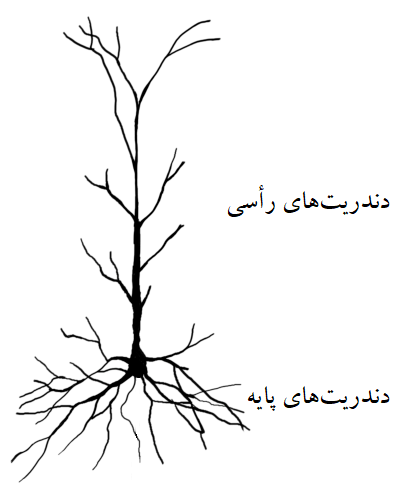
\includegraphics[width=0.5\linewidth]{pyramidal.png}
		\caption[NS]{
			نمایی از ساختار یک نورون هرمی و دندریت‌های رأسی و قاعده‌ای در آن.
		}
		\label{fig:pyramidal}
	\end{figure}
	
	\section{\gls{snn}}
	\gls{ann}\LTRfootnote{Artificial Neural Networks} بر پاییه‌ی دینامیک‌های بسیار ساده‌شده مغز ساخته شده‌اند و به عنوان یک ابزار محاسباتی قوی برای حل بسیاری از مسائل استفاده می‌شوند
	\cite{TGNN}. 
	\gls{snn}\LTRfootnote{Spiking Neural Networks} نوعی از شبکه‌های عصبی مصنوعی هستند که در آن ارتباط بین نورون‌ها توسط ضربه‌ها و سیناپس‌ها  با وزن‌های متغیر، مطابق با مشاهدات زیستی تعریف شده‌اند
	\cite{ghosh2009spiking}. 
	از جمله مهمترین ویژگی‌هایی که در \gls{snn} در نظر گرفته‌شده، بعد زمان است
	\cite{Mozafari2019}
	که شبکه‌های عصبی کلاسیک فاقد این ویژگی بوده‌اند. در \gls{snn} اطلاعات می‌توانند در زمان‌های مختلفی منتقل شوند و خود زمان در مفهوم منتقل‌شده نقش مهمی را بازی می‌کند
	\cite{SNN1997}.
	
	برای شبیه‌سازی این گونه از شبکه‌های عصبی، سازوکار نورون‌های زیستی به روش‌‌های گوناگونی مدل‌سازی شده‌، که در ادامه به آن‌ها اشاره خواهد شد.
	% که ازجمله ساده‌ترین‌ آن‌ها، که در عین‌ حال کارایی بسیار مناسبی نیز دارد، مدل نورونی \gls{lif}\LTRfootnote{Leaky integrate-and-fire} است که در ادامه به آن خواهیم پرداخت.
	
	\subsection{مدل‌های نورونی}
	از اولین تلاش‌های صورت گرفته برای مدل‌سازی نورون‌ها می‌توان به مدل ارائه شده توسط هاجکین و هاکسلی اشاره کردد که حاصل تحقیقات و آزمایش‌های آن‌ها روی ماهی‌مرکب است \cite{Hodgkin1952}. این مدل، به دلیل لحاظ شدن بسیار دقیق فرآیند‌ها در آن، از دقت بسیار بالایی برخوردار است که در عوض از نظر محاسباتی هزینه‌ی زیادی دارد. به همین دلیل مدل‌های نورونی دیگری نیز پس از آن ارائه شدند که در سازوکار‌های آن‌ها ساده‌سازی انجام شده و از دقت کمتری برخوردار هستند، ولی در عوض هزینه‌ی محاسباتی بسیار کم‌تری دارند. 
	
	از دیگر مدل‌های نورونی ارائه شده، مدل نورونی ایزیکویچ\LTRfootnote{Izhikevich} است که در آن تلاش شده با ارائه‌ی ساز‌وکاری کاملاً متفاوت از نورون‌های زیستی، مدلی با هزینه‌ی محاسباتی بسیار کم، در عین امکان رخ دادن طیف وسیعی از الگو‌های رفتاری نورون‌های زیستی در آن، ارائه شود \cite{1257420}. هرچند، در بسیاری از موارد از این مدل نورونی به دلیل تفاوت با مدل زیستی در مدل‌سازی‌ها استفاده نمی‌شود.
	
	یکی دیگر از مدل‌های نورونی مورد استفاده در مدل‌سازی‌ها مدل نورونی 
	\gls{lif}
	است که یک مدل مبتنی بر سازوکار نورون‌های زیستی است که بسیار ساده‌سازی شده است ولی در عین حال رفتار قابل قبولی دارد. این مدل با وجود هزینه‌ی محاسباتی بسیار کم، بر خلاف مدل ایزیکویچ، سازوکاری مشابه نورون زیستی دارد که در بخش بعدی به شرح کامل‌تر این مدل نورونی خواهیم پرداخت.
	
	\subsection{مدل نورونی \gls{lif}}
	در مدل نورونی \gls{lif} تلاش شده‌است تا ویژگی‌ها و خواص مهم نورون‌های زیستی لحاظ شوند. در این مدل‌نورونی، با وارد‌شدن ضربه‌های تولیدشده توسط نورون‌های پیش‌سیناپسی به نورون مد ‌نظر، اختلاف پتانسیل آن افزایش می‌یابد (تجمیع) و در صورت رسیدن اختلاف پتانسیل به یک آستانه‌ی مشخص، این نورون ضربه‌ای تولید می‌کند (آتش) که توسط اتصالات بین نورونی به نورون‌های پس‌سیناپسی منتقل می‌شود. همچنین در گذر زمان اختلاف پتانسیل نورون به‌مرور در حال کاهش به سمت یک میزان مشخص اختلاف پتانسیل است (نشتی) که به آن اختلاف پتانسیل استراحت می‌گوییم
	\cite{gerstner2014neuronal}.
	
	ساز‌وکار تغییرات اختلاف پتانسیل را در این مدل نورونی می‌توان به صورت معادله‌ی دیفرانسیل بیان‌شده در رابطه‌ی \ref{eq:lif} نوشت:
	\cite{gerstner2014neuronal}.
	
	\begin{align}
		\tau . \frac{du}{dt} = -(u - u_{rest}) + R . I(t) 
		\label{eq:lif}
	\end{align}

 در رابطه‌ی فوق، $u$ اخلاف پتانسیل فعلی نورون، $u_{rest}$ اختلاف \gls{rest}، $I(t)$ جریان ورودی به نورون و $R$ مقاومت الکتریکی قشای نورون را نشان می‌دهند


\subsection{انعطاف‌پذیری نورونی}

\gls{Neuroplasticity}\LTRfootnote{Neuroplasticity} را می‌توان به عنوان توانایی سیستم عصبی برای تغییر فعالیت خود در پاسخ به محرک‌های درونی یا بیرونی با اعمال تغییراتی در ساختار، عملکرد و اتصالات خود قلمداد کرد~\cite{MateosAparicio2019}.
همچنین می‌توان پدیده‌ی یادگیری در موجودات زنده را محصول وجود انعطاف‌پذیری نورونی در آن‌ها دانست.

از میان تأثیراتی که در نتیجه‌ی انعطاف‌پذیری نورونی ایجاد می‌شود، می‌توان به تغییر میزان تأثیر تحریکی یا مهاری \gls{pre} روی \gls{post} اشاره کرد که در نتیجه‌ی تغییر در ساختار دندریت‌ها و آکسون‌ها رخ می‌دهد.
از جمله مهم‌ترین ‌قوانین یادگیری در این خصوص، \gls{hebb}‌\LTRfootnote{H‌ebbian Learning Rule} است که به واسطه‌ی فعالیت‌های دونالد هب\LTRfootnote{Donald Hebb} معرفی شده‌است.
\gls{hebb} به این صورت بیان شده‌است: «زمانی که آکسون نورون \emph{الف} به اندازه‌ای به (دندریت) نورون \emph{ب} نزدیک  باشد که مکرراً یا دائماً باعث تحریک آن شود، برخی فر‌آیند‌ها و تغییرات متابولیکی در یک یا هر‌دوی نورو‌ن‌ها باعث تغییراتی می‌شوند تا تأثیر نورون \emph{الف} در تحریک نورون \emph{ب} افزایش یابد»
\cite{hebb1949organization}.
همچنین کارلا شاتز\LTRfootnote{Carla Shatz} این‌گونه قانون هب را تفسیر می‌کند: «نورون‌هایی که هم‌زمان ضربه می‌زنند، به ‌هم متصل می‌شوند»
\cite{shatz1992developing}.
این تفسیر ممکن است باعث برداشت غلط شود، چراکه اگر دو نورون به معنی واقعی کلمه در یک لحظه شلیک کنند، امکان این‌که شلیک یکی از آن نورون‌ها معلول شلیک نورون دیگر باشد وجود نخواهد داشت. بیشتر از موضوع هم‌زمانی، موضوع ارتباط علت و معلولی بین شلیک نورون‌ها است که دارای اهمیت می‌باشد
\cite{granger1969investigating}.


در دهه‌ی ۱۹۹۰ میلادی، نتایج حاصل از آزمایش‌ها باعث مشخص‌شدن پایه‌های نوروفیزیولوژیک قانون هب بر اساس \gls{stdp}\LTRfootnote{Spike-timing dependent plasticity (STDP)} شدند~\cite{caporale2008spike}.
در این آزمایش‌ها مشخص شد وقتی یک \gls{exc}، به یک نورون تحریکی دیگر متصل شده‌باشد، اگر \gls{pre} با فاصله‌ی زمانی ۴۰ میلی‌ثانیه یا کمتر نسبت به \gls{post} ضربه بزند، سیناپس‌های مرتبط با اتصال آن‌ها تقویت می‌شوند و اگر \gls{post} زودتر از \gls{pre} ضربه بزند، سیناپس‌های مرتبط با اتصال آن‌ها تضعیف خواهند شد (شکل \ref{fig:stdp}).
بر اساس روابط کشف‌شده در تضعیف و تقویت سیناپس‌ها، می‌توان تغییرات میزان اثرگذاری نورون‌ها روی یکدیگر را به صورت زیر مدل‌سازی کرد~\cite{gerstner2014neuronal}:
\begin{align}
	\Delta w =
	\begin{cases}
		A_+(w).\exp(\frac{-|\Delta t|}{\tau_+})  & \text{\lr{if}}\; t_{pre} \leq t_{post}, \\
		A_-(w).\exp(\frac{-|\Delta t|}{\tau_-})  & \text{\lr{if}}\; t_{pre} > t_{post}.
	\end{cases}
	\label{eq:stdp}
\end{align}

در این‌جا $w$ میزان اثرگذاری یک نورون روی نورون دیگر، $\tau_\pm$ ثابت‌های زمانی  و $A_\pm$ میزان تغییرات وزن‌های سیناپسی هستند.

\begin{figure}[H]
	\centering
	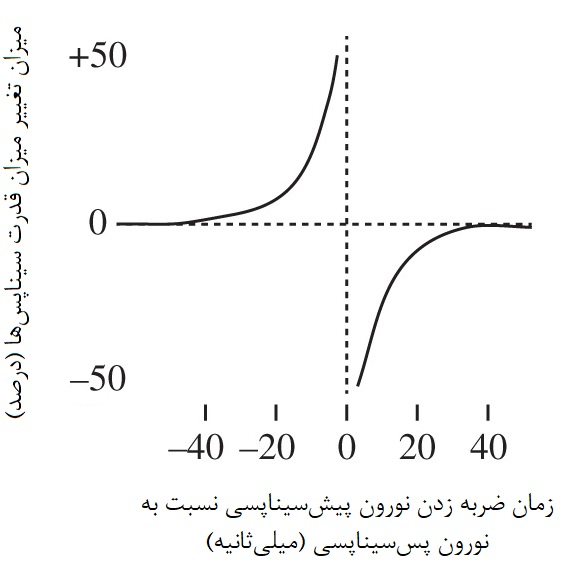
\includegraphics[width=0.6\linewidth]{stdp.jpg}
	\caption[NS]{
		میزان تغییرات سیناپس‌ها در \gls{stdp} در فواصل زمانی مختلف برای اتصالات بین نورون‌های تحریکی.
	}
	\label{fig:stdp}
\end{figure}

همچنین از آن زمان تا کنون مشخص شده که این الگوی تغییرات برای سیناپس‌های مهاری متفاوت است و تغییرات وزن در هنگامی که فاصله‌ی زمانی بین ضربه‌زدن \gls{pre} و \gls{post} از حدود ۵ میلی‌ثانیه کمتر باشد، بسیار ناچیز خواهد بود که در شکل \ref{fig:stdp-inh} نمایش داده شده‌است~\cite{Haas2006}.

\begin{figure}[H]
	\centering
	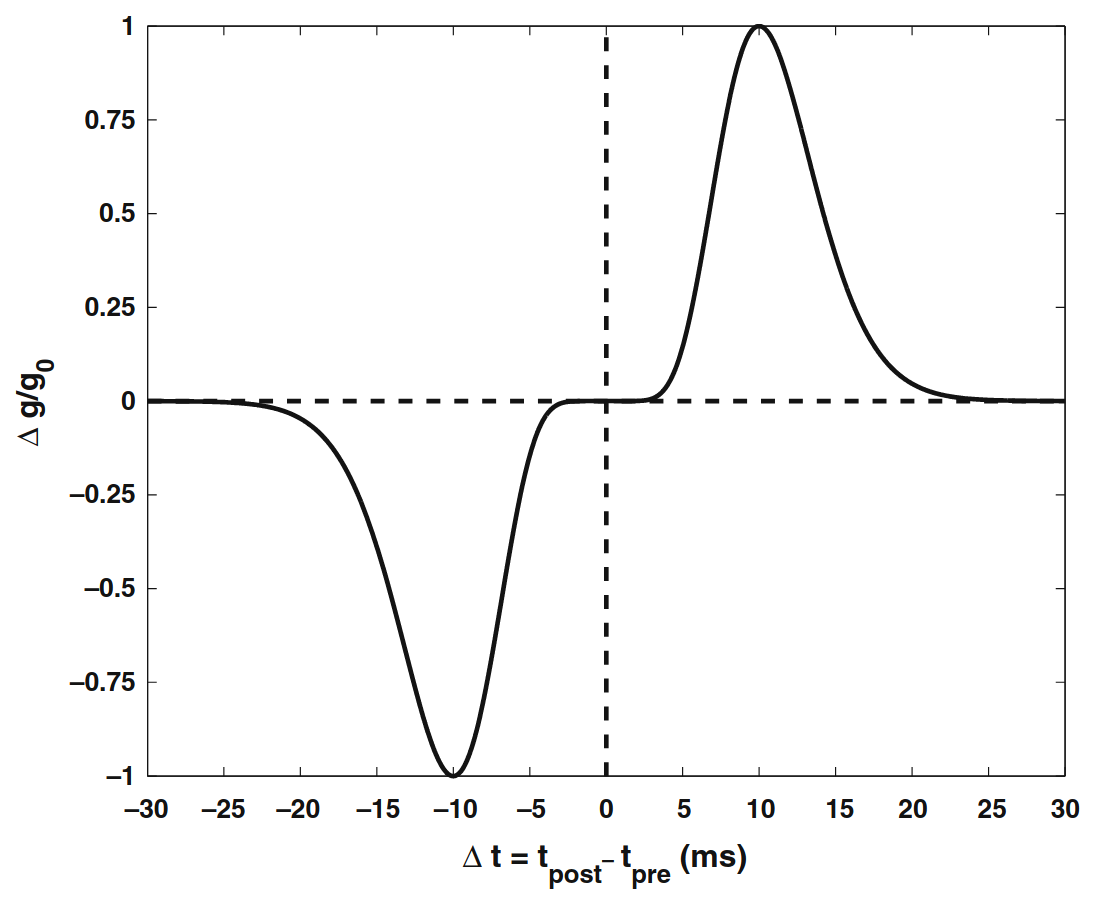
\includegraphics[width=0.7\linewidth]{stdp-inh.png}
	\caption[NS]{
		میزان تقویت سیناپس‌ها در \gls{stdp} در فواصل زمانی مختلف برای \gls{synapse}‌های مهاری.
	}
	\label{fig:stdp-inh}
\end{figure}

\subsection{سازوکار پاداش در مغز}
\label{section:reward-in-brain}

بخش بزرگی از یادگیری انسان در تعامل با محیط اتفاق می‌افتد. هر خروجی انسان تأثیری روی محیط پیرامونش گذاشته و محیط تغییر‌یافته، خود به عنوان یک درون‌داد از طریق سیستم عصبی محیطی درک می‌شود
\cite{sutton1998reinforcement}.
با توجه به درک انسان از محیط، پاداش یا تنبیه نیز برای آن در نظر گرفته می‌شود که این ساز‌و‌کار در مغز انسان بر عهده‌ی پیام‌رسان‌های عصبی\LTRfootnote{Neurotransmitter}  مانند \gls{dopamine}\LTRfootnote{Dopamine} است. 

\begin{figure}[H]
	\centering
	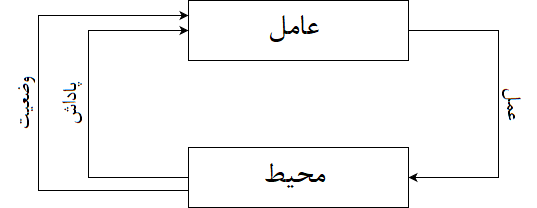
\includegraphics[width=0.7\linewidth]{rl.png}
	\caption[NS]{
		آثار \gls{agent} و محیط بر روی یکدیگر
	}
	\label{fig:rl}
\end{figure}

تأثیر پاداش روی فعالیت نورون‌ها به این صورت است که برخی از نورون‌ها به این دسته از پیام‌رسان‌‌های عصبی حساس هستند و میزان غلظت آن‌ها روی فعالیت این دسته از نورون‌ها تأثیر‌گذار است و این تأثیر به گونه‌ای است که در صورت دریافت سیگنال پاداش، تغییرات وزن‌های اتصالات نورونی مشابه \gls{stdp} تغییر خواهند کرد؛ هرچند که میزان پاداش در شدت این تغییرات موثر است. همچنین در صورتی که سیگنال تنبیه دریافت شود تغییرات وزن‌های اتصالات بین نورونی برعکس \gls{stdp} تغییر خواهند کرد و میزان این تغییرات به طور مشابه، وابسته به میزان شدت تنبیه خواهد بود.

برای مدل‌سازی اثر سازوکار پاداش روی یادگیری می‌توان از روابط زیر استفاده کرد~\cite{gerstner2014neuronal}:  
\begin{subequations}
	\begin{align}
		\frac{dc}{dt} &= -\frac{c}{\tau_c} + STDP(\tau) \delta(t-t_{pre/post}) \label{eq:rstdp1}\\
		\frac{dd}{dt} &= -\frac{d}{\tau_d} + DA(t) \label{eq:rstdp2}\\
		\frac{ds}{dt} &= cd
		\label{eq:rstdp3}
	\end{align}
\end{subequations}

در روابط فوق، $d$ میزان دوپامین (پاداش)، $\delta$ تابع دیراک، $\tau_c$ و $\tau_d$ به عنوان ثابت‌های زمانی و $DA$ به عنوان تابع دوپامین ترشح‌شده در نظر گرفته‌ شده‌اند.



	\subsection{\gls{rl} در شبکه‌های عصبی ضربه‌ای}
	
	یادگیری تقویتی یکی از روش‌های آموزش دادن عامل‌های هوشمند است، که در آن عامل هوش‌مند با آزمون و خطا و با دریافت بازخورد از محیط خود، آموزش داده می‌شود تا به گونه‌ای رفتار کند تا به صورت مفیدتری با محیط تعامل داشته باشد. به عبارتی عامل می‌آموزد تا به گونه‌ای رفتار کند تا بیشترین پاداش را از محیط دریافت کند. در یادگیری تقویتی هیچ نظارتی بر روی عامل وجود ندارد و عامل خود باید در تعامل با محیط و آزمون و خطا رفتار بهینه را بیاموزد.
	
	پیش‌تر در بخش \ref{section:reward-in-brain} به سازوکار پاداش در مغز انسان پرداختیم و مدل آن را نیز بررسی کردیم (روابط \ref{eq:rstdp1}، \ref{eq:rstdp2} و \ref{eq:rstdp3}). از سازوکار مطرح‌شده در \gls{snn} برای یادگیری تقویتی استفاده می‌شود تا مدل با توجه به الگوی فعالیتش در طول زمان و در مجاورت محیط، که منجر به دریافت پاداش و تنبیه می‌شود، آموزش داده شود و رفتار آن به سمتی متمایل شود که بیشترین پاداش را در طول زمان دریافت کند. قانون یادگیری حاصل از استفاده از این مدل را \gls{rstdp}\LTRfootnote{Reward-modulated spike-timing dependent plasticity} می‌نامند.
	
	برای به‌کار‌گرفتن یادگیری تقویتی در یک مدل، باید بر اساس شرایط محیط فرضی شبیه‌سازی شده و برای رفتار عامل در آن، یک مقدار پاداش یا تنبیه محاسبه شود تا بتوان به عنوان مقدار دوپامین در مدل از آن استفاده کرد.
 	
 	
	\subsection{جمعیت‌های نورونی}
	نورون‌ها در مغز به صورت گروه‌هایی قابل تقسیم‌بندی هستند؛ همچون انواع مختلف نورون‌ها، لایه‌های قشر مغزی یا ستون‌های قشری. در مدل‌سازی‌ها نیز به جای استفاده از تعداد بسیار زیادی از تک نورون‌های شبیه‌سازی‌شده، نورون‌ها در مجموعه‌هایی دسته‌بندی شده و مجموعه‌ای از نورون‌ها همراه با یکدیگر بررسی می‌شوند. 
	
	یکی از مواردی که برای یک جمعیت نورونی قابل محاسبه است، فعالیت جمعیت نورونی است که به صورت یک نسبت از تعداد ضربه‌ها در بازه‌های زمانی کوتاه مدت تعریف می‌شود. فعالیت یک جمعیت نورونی در زمان $t$ به صورت زیر تعریف می‌گردد:
	
	\begin{align}
		A(t) = \frac{1}{\Delta t} \frac{n_{act}(t; t+\Delta t)}{N}
		\label{eq:stdp}
	\end{align}
	
	در رابطه‌ی فوق $\Delta t$ بازه‌ی زمان شمارش ضربه‌ها،
	$n_{act}(t; t+\Delta t)$
	تعداد ضربه‌ها در بازه‌ی زمانی $t$ تا $t + \Delta t$ و $N$ تعداد نورون‌های جمعیت نورونی مورد بررسی است.
	
	جمعیت‌های نورونی به دو صورت متفاوت قابل تعریف هستند: جمعیت‌هایی‌ که متشکل از نورون‌های یکسان، که به آن‌ها \gls{homogenpop}\LTRfootnote{Homogeneous Populations} گفته می‌شود، و جمعیت‌هایی که متشکل از نورون‌های غیریکسان هستند که به آن‌ها \gls{hetrogenpop}\LTRfootnote{Heterogeneous Populations} گفته می‌شود.
	
	همچنین‌ اتصالات بین جمعیت‌های نورونی نیز باید برقرار شود. برای این منظور می‌توان به دو حالت کلی اتصال دو جمعیت نورونی را تعریف کرد: اتصال کامل و اتصال تصادفی. در اتصال کامل هر نورون در جمعیت پیش‌سیناپسی به هر نورون در جمعیت پس‌سیناپسی متصل است. ولی در اتصال تصادفی یا میزان اتصالات بین نورون‌های جمعیت‌های پیش‌سیناپسی و پس‌سیناپسی به صورت تصادفی مشخص می‌شود، یا این‌که تعداد اتصالات عددی ثابت در نظر گرفته شده و این مسئله که هر نورون پیش‌سیناپسی به کدام نورون‌های پس‌سیناپسی متصل شوند به صورت تصادفی مشخص می‌گردد.
	
	\chapter{طرح مسئله}
	
	در این فصل پس از یک مرور مختصر درباره‌ی مسئله‌ی \gls{binding} به اهمیت مدل‌سازی مسئله‌ی \gls{binding} و مسائلی که درک بیشتر ما از این موضوع آن‌ها را نیز تحت تأثیر قرار خواهد داد، خواهیم پرداخت. از میان این مسائل، می‌توان به هوش مصنوعی و درک بهتر ساز‌وکار مغز اشاره کرد.
	
	\section{مسئله‌ی \gls{binding}}
	
	در حوزه‌های علوم اعصاب، علوم شناختی و فلسفه‌ی ذهن مسئله‌ای تحت عنوان مسئله‌ی \gls{binding}
	\LTRfootnote{Binding Problem}
	یا \gls{combprob}
	\LTRfootnote{Combination Problem}
	مطرح می‌شود که به چگونگی پردازش و درهم‌آمیختن مفاهیم مختلف مجزا از هم، همچون اشیاء و ویژگی‌های انتزاعی و احساسی، به صورت یک مفهوم تجمیع‌شده‌ی گسترده‌تر و درک آن‌ها به صورت یک تجریه‌ی واحد می‌پردازد
	\cite{REVONSUO1999123, Feldman2012} (تصویر \ref{fig:binding-neuron} و \ref{fig:binding}).
	به دلیل این‌که هنوز به صورت کامل از سازوکار \gls{binding} اطلاعی در دست نیست، از آن به عنوان یک مسئله یاد می‌شود.
	
	\begin{figure}[]
		\centering
		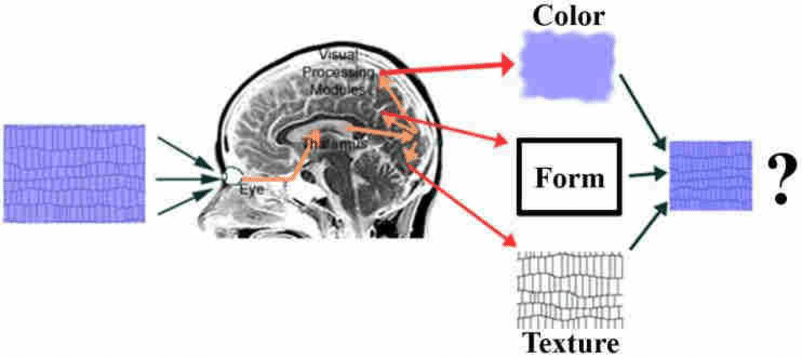
\includegraphics[width=1.0\linewidth]{binding-neuron.png}
		\caption[NS]{
			یک مثال از چگونگی ادراک یک تصویر شامل رنگ، طرح و چارچوب توسط مغز. تصویر به صورت کلی توسط ورودی‌های حسی وارد مغز می‌شود و ویژگی‌های آن (رنگ، طرح و حالت) به صورت مجزا درک می‌شوند. نهایتاً یک مفهوم جامع شامل تمام ویژگی‌های تصویر، از مفاهیمی که به صورت مجرا درک شده‌بودند، شکل می‌گیرد \cite{Masi2021-rv}.
		}
		\label{fig:binding-neuron}
	\end{figure}
	
	\begin{figure}[]
		\centering
		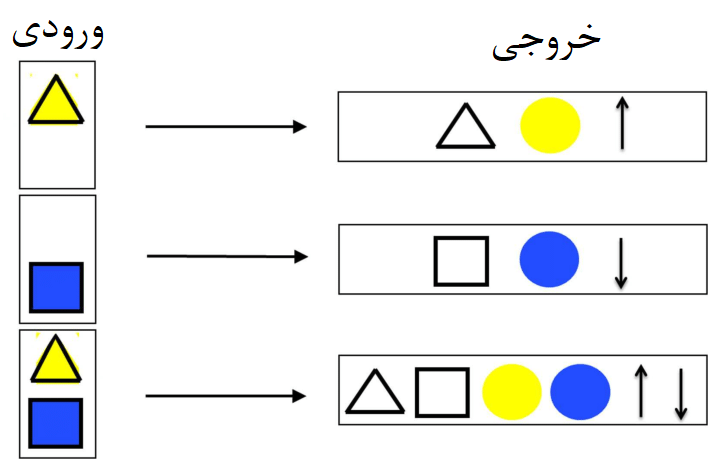
\includegraphics[width=0.7\linewidth]{binding.png}
		\caption[NS]{
			یک نمایش از تعریف کلاسیک \gls{binding} و چگونگی ادراک مفاهیم جامع توسط درک مفاهیم جزئی‌تر.
			\cite{velic2012}.
		}
		\label{fig:binding}
	\end{figure}
	
	به صورت کلی مسئله‌ی انقیاد توضیحی برای ظرفیت ما در یکپارچه‌کردن اطلاعات در طول زمان، فضا، ویژگی‌های مختلف و ایده‌ها است. مسئله‌ی انقیاد به صورت سه موضوع مجزا قابل بررسی است و در هر یک از تحقیقات مختلف، مسئله‌ی انقیاد به یکی از این سه موضوع تعلق می‌یابد~\cite{Treisman1999}:
	
	\begin{enumerate}
		\item چگونگی تشخیص مفاهیم مقید‌شده به عنوان یک مفهوم واحد  و تفکیک آن‌ها از مفاهیمی که مقید به مفاهیمی دیگر هستند.
		\item چگونگی کد‌گذاری انقیاد در مغز و این‌که چگونه در مغز به آن رجوع می‌شود.
		\item چگونگی تشخیص ارتباط صحیح بین مفاهیم  مقید‌شده و یک شی بخصوص.
	\end{enumerate}

	بسیاری از پژوهش‌های مرتبط با مسئله‌ی انقیاد در موضوع دوم هستند. در پژوهش حاضر نیز مفهوم مورد بررسی، چگونگی رخدادن انقیاد در مغز و در مقیاس ارتباطات نورونی است که به دسته‌ی دوم، یعنی چگونگی کدگذاری  در مغز مرتبط می‌شود \cite{Treisman1999}. درواقع مسئله‌ی اصلی چگونگی یکپارچه‌شدن مفاهیم مجزا ولی مرتبط در قالب یک مفهوم واحد در ساختار نورون‌ها و اتصالات بین آن‌ها است.
	برای نمونه، انسان در صورت قرار گرفتن در مجاورت یک خودرو از طریق حس بینایی، تصویر خودرو و از طریق حس شنوایی صدای خودرو را درک می‌کند. تصویر خودرو و صدای خودرو در مغز در موقعیت‌های مختلفی درک شده و نورون‌های آن بخش‌ها به این ورودی‌ها حساس می‌شوند. ولی هم‌زمانی تجریه‌ی این دو مفهوم باعث شکل گیری یک مفهوم سطح بالاتر و انتزاعی از خودرو می‌شود که موجب می‌شود فرد بتواند یک مفهوم شامل صدا و تصویر از خودرو را درک کند.


\section{شواهد رخدادن \gls{binding} در مغز انسان}
\label{subsection:binding-in-human}


آنه تریسمن\LTRfootnote{Anne Treisman}
و هیلاری اشمیت\LTRfootnote{Hilary Schmidt}
آزمایشی را انجام دادند که در آن به مطالعه‌ی اثری با نام \gls{illcon}\LTRfootnote{Illusory Conjunctions}
پرداختند که در آن ویژگی‌های یک شئ به شئ دیگری منتسب می‌شود
\cite{TREISMAN1982107}.
بر اساس نظر تریسمن، علت این انتصاب اشتباه در ویژگی‌های اشیاء، حضور جدا از هم صفات در مراحل اولیه‌ی ادراکی است
\cite{goldstein_2019}.
اهمیت این موضوع از این جهت است که دیگر حالت ممکن آن است که یک شئ، نه به صورت صفات جداگانه، بلکه به صورت یک ماهیت کامل حاضر شود. این در حالی است که رخدادن مسئله‌ی \gls{binding} در مغز مستلزم حضور ویژگی‌ها و صفات به صورت جدا از هم می‌باشد که این آزمایش نشانگر اتفاق‌افتادن \gls{binding} در مغز است. همچنین گروهی دیگر برای نشان دادن مصادیق انقیاد در انسان به نمونه‌های شناختی آن همچون \gls{Bind}‌کردن دانش معنایی\LTRfootnote{Semantic Knowledge} به شهود، مقیدکردن متغیر‌ها در زبان و استنتاج اشاره می‌کنند \cite{greff2020binding}.


\section{تعریف مسئله}
همواره شبیه‌سازی و درک ساختار‌های موجود در مغز انسان جزو مسائل مورد اهمیت برای بشر بوده‌است و در دهه‌های اخیر نیز با رشد و گسترش قدرت محاسباتی و علومی چون هوش مصنوعی و علوم اعصاب این اهداف بسیار دردسترس‌تر از پیش به نظر می‌رسند. فعالیت‌های بسیاری نیز در دهه‌های اخیر در رابطه با این موضوع آغاز شده‌است که از جمله‌ی آن‌ها می‌توان به پروژه مغز آبی\LTRfootnote{Blue Brain Project} و پروژه‌ی مغز انسان\LTRfootnote{Human Brain Project (HBP)} اشاره کرد.

چنانچه پیش‌تر مطرح شد، مسئله‌ی \gls{binding} به عنوان یکی از مهمترین مسائل در شناخت مغز و هوش مصنوعی، که تقریباً در تمام فعالیت‌های شناختی پستانداران در حال رخدادن است، برای شبیه‌سازی در شبکه‌های عصبی مصنوعی کلاسیک که صرفاً نرخ ضربه را کد می‌کنند\LTRfootnote{Rate-coding} با محدودیت‌هایی مواجه است \cite{vonderMalsburg1999} که این موضوع را در دسته‌ی مسائل حل‌نشده قرار داده‌است. ولی در سال‌های اخیر با افزایش قدرت پردازشی و پیشرفت شبکه‌های عصبی ضربه‌ای‌، امید است تا بتوان با استفاده از این نسل از شبکه‌های عصبی مصنوعی مسیر جدیدی را در درک و شبیه‌سازی مسئله‌ی \gls{binding} در پیش گرفت و به نتایج بهتری نسبت به انواع کلاسیک در آن رسید.

همچنین استفاده از شبکه‌های عصبی ضربه‌ای این امکان را برای ما فراهم می‌کند که در ساختار و توپولوژی شبکه نیز از ساختار‌های طبیعی مغز بیش از پیش الگوبرداری کنیم. این موضوع از این جهت  حائز اهمیت است که \gls{binding} در مغز پستانداران در حال رخدادن است و هرچه بیشتر سازوکارها و شبکه‌ی شبیه‌سازی‌شده مشابه نمونه‌ی طبیعی خود باشند احتمال رخدادن \gls{binding} نیز در شبیه‌سازی بیشتر خواهد بود.

در مطالعه‌ی پیش‌رو در تلاش خواهیم بود تا با استفاده از شبکه‌های عصبی ضربه‌ای و الگوبرداری از ساختار و توپولوژی مغز پستانداران یک شبکه‌ی عصبی را شبیه‌سازی کرده و در آن وجود آثاری از رخدادن \gls{binding} را بررسی کنیم.


	
	\section{چالش‌های موجود}
	در زمینه‌ی شبکه‌های عصبی، مسئله‌ی انقیاد تنها یک مسئله‌ی حل‌نشده درباره‌ی ادراک نیست، بلکه تشخیص محدودیت‌های حال حاضر شبکه‌های عصبی مصنوعی موجود نیز بخشی از مسائلی است که محققان را مشغول خود کرده‌است.
	با توجه به چالش‌های کنونی، درک چگونگی رخداد \gls{binding} در مغز، از اهمیت بالایی برخوردار است؛ زیرا با توجه به اهمیت و میزان تأثیر \gls{binding} در آگاهی و درک موجود زنده از محیط خود، به این موضوع در مسائلی همچون درک و شبیه‌سازی هوش انسانی که یکی از چالش‌های هوش مصنوعی است، نیاز است.
	
	 فعالیت‌های بسیاری در راستای دست‌یابی به سیستم‌های هوشمند انجام شده‌است که از جمله‌ موفق‌ترین و موثر‌ترین روش‌های حاضر، استفاده از شبکه‌های عصبی مصنوعی است که یک روش الهام گرفته‌شده از \gls{nervousSystem} انسان است و این شبکه‌ها در حال حاضر به صورت گسترده مورد استفاده قرار گرفته‌اند. این روش در  عین این‌که در شرایط مناسب از بهره‌وری بسیار خوبی برخوردار است و امکان دست‌یابی به نتایج بسیار خوبی را در مدل‌سازی آماری داده‌های جهان دارد، به میزان داده‌ی بسیار زیادی برای آموزش نیاز دارد، در انتقال مفاهیم از پیش آموخته‌شده به مسائل جدید نیز با مشکل مواجه است و امکان عمومی‌سازی مسائل آموخته‌شده را ندارد.
	از جمله اصلی‌ترین مشکلات و محدودیت‌های موجود در شبکه‌های عصبی مصنوعی، ناتوانی آن‌ها در شکل‌دهی، بازنمایی و ارتباط بین مفاهیم و موجودیت‌ها است. به خوبی نشان داده شده‌است که درک انسان حول اشیاء شکل گرفته‌است. این اشیاء می‌توانند به صورت مستقل پردازش شده و به حالت‌های بسیار زیادی دوباره با یکدیگر ترکیب شوند. این مسئله به انسان امکان تعمیم درک خود به مسائل فراتر از تجربیاتش را می‌دهد و این ساز‌وکار همان رویه‌ی مورد بررسی در مسئله‌ی \gls{binding} است
	\cite{greff2020binding}.
	
	ارتباطات بین مفاهیم در رخدادن انقیاد به شکل‌های مختلفی ممکن است؛ همچون رابطه‌ی علّی، ارتباط سلسه‌مراتبی و ارتباط مقایسه‌ای. تعریف مفاهیم در قالب انواع مختلف این روابط می‌تواند تأثیراتی روی مفاهیم شکل گرفته داشته‌باشد. همچنین نکته‌ی مهم‌ این است که این روابط به صورت مجزا از هم و مستقل از مفاهیم شکل‌گرفته‌ از اشیا باشند. انواع مختلف ارتباطات قابل پیاده‌سازی نیز، خود یکی از چالش‌های موجود در حل این مسئله است.
	
	\section{دلایل استفاده از شبکه‌های عصبی ضربه‌ای در مسئله‌ی انقیاد}
	شبکه‌های عصبی ضربه‌ای در مقایسه با شبکه‌های عصبی کلاسیک از توجیه زیستی بسیار بیشتری برخوردار هستند و در آن‌ها جزئیات نورون‌های زیستی بسیار بیشتر در نظر گرفته‌شده‌است که این موضوع پتانسیل‌های این دسته از شبکه‌هارا نیز تحت تأثیر قرار می‌دهد. در این دسته از شبکه‌ها به دلیل انتقال داده‌ها با در نظر‌گرفتن زمان و در قالب ضربه (به جای عدد در شبکه‌‌های عصبی کلاسیک) امکان درک مفاهیم به صورت اشیاء به جای مدل‌سازی آماری در آن‌ها بسیار محتمل‌تر است و به همین دلیل این امکان وجود دارد که بتوان در این دسته از شبکه‌های عصبی، سازوکاری را تحت شرایط مشخصی به‌وجود آورد که در آن مسائل و مشکلات مطرح‌شده دیگر رخ ندهند و به عبارتی در این دسته از شبکه‌های عصبی می‌توان انتظار رخداد \gls{binding} را داشت.
	
	\chapter{تحقیقات پیشین}
	
	در این فصل مجموعه‌ای از تحقیقات انجام‌شده پیرامون مسئله‌ی \gls{binding} و نظریه‌هایی پیرامون چگونگی رخدادن آن در مغز و تلاش‌هایی برای مدل‌سازی آن به صورت محاسباتی را بررسی خواهیم کرد.
	
	\section{رخدادن انقیاد در مغز انسان}
	همان‌طور که در بخش \ref{subsection:binding-in-human} نیز اشاره شد، تحقیقی توسط آنه تریسمن و هیلاری اشمیت صورت گرفته که نشان می‌دهد ویژگی‌های مختلف یک شی در مغز به صورت مجزا از هم پردازش می‌شوند~\cite{TREISMAN1982107}.
	آن‌ها صفحه‌ای را به شرکت‌کننده ارائه می‌کردند که در آن چهار شکل با رنگ‌های مختلف به همراه دو عدد مشکی وجود داشت. آن‌ها این صفحه را به مدت $0.2$ ثانیه نشان می‌دادند و پس از آن یک صفحه با نقاط مشکی تصادفی نمایش داده می‌شد. هدف از نمایش صفحه با نقاط مشکی، از بین بردن هر نوع رد ادراکی از محرک پیشین بود. سپس از شرکت‌کنندگان خواسته می‌شد تا اعداد و اشکال نمایش‌داده‌شده را توصیف کنند.
	
	در حدود یک‌پنجم کوشش‌های شرکت کنندگان، ترکیب‌شدن ویژگی‌های اشکال نمایش داده شده دیده می‌شد. برای مثال رنگ یا اندازه‌ی دو شکل با یکدیگر جابه‌جا گزارش می‌شدند.
	بر اساس نظر تریسمن، علت شکل‌گیری این پدیده، جدا‌بودن صفات از یکدیگر در مرحله‌ی پیش‌توجهی و مقید‌نبودن آن‌ها به شی‌ به‌خصوصی است \cite{goldstein_2019}.
	
	\section{پیدایش \gls{binding} در گروه‌های چندزمانی}
	اگوچی و همکارانش در پژوهشی
	\cite{EGUCHI2018a}
	با ساخت یک شبکه‌ی عصبی سلسله‌مراتبی که لحاظ‌کردن تاخیر انتقال آکسونی\LTRfootnote{Axonal Transmission Delay} در آن باعث شده تا در زیرجمعیت‌های آن \gls{polychron}\LTRfootnote{Poly-chron Groups}\cite{Izhikevich2006-dy} شکل بگیرند که هر یک از آن‌ها به یک الگوی تصادفی با توزیع \gls{poisson} حساس شده‌بودند، نشان دادند که \gls{binding} بین مفاهیم دیداری سطح پایین و سطح بالا به‌مرور زمان شکل می‌گیرد که در این شبکه هر یک از این مفاهیم در قالب فعالیت یک گروه چندزمانی در نظر گرفته‌ شده‌بودند.
	
	مثالی از نمود بسیار ساده‌ی \gls{binding} در این شبکه در شکل \ref{fig:eguchi-binding} نشان داده شده‌است که در آن به دلیل وجود تاخیر در انتقال، وقتی چند مفهوم که هر کدام به یک یا مجموعه‌ای از نورون‌ها مقید‌ شده‌اند، در فواصل زمانی مشخصی به شبکه داده شوند باعث فعال‌شدن یک مفهوم سطح بالاتر که شامل مفاهیم سطح پایین‌تر نیز می‌باشد، می‌گردند.
	
	\begin{figure}[H]
		\centering
		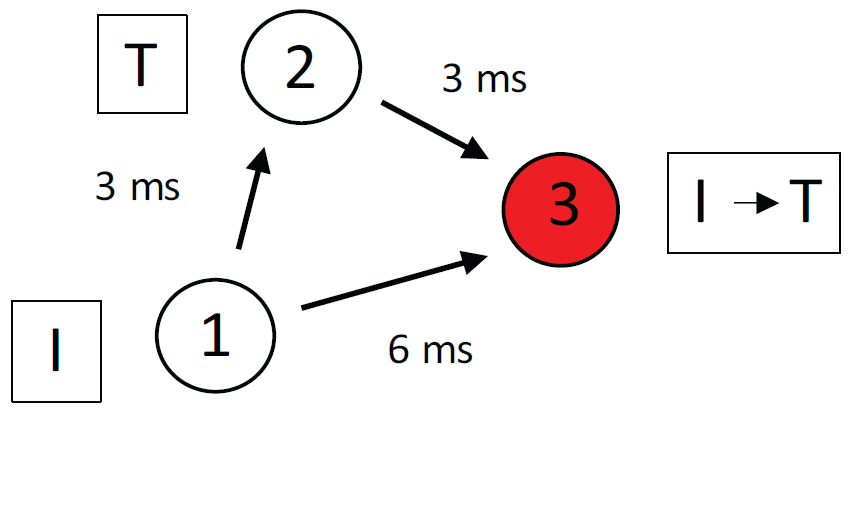
\includegraphics[width=0.6\linewidth]{poly-bind.png}
		\caption[NS]{
			یک مثال فرضی از انقیاد در سطح نورونی که در آن نورون شماره‌ی ۱، یک ویژگی سطح پایین مثل یک خط عمودی را نمایندگی می‌کند و نورون شماره ۲ نیز یک ویژگی سطح بالاتر مثل تصویر حرف T را نمایندگی می‌کند و نورون شماره ۳ انقیاد را مشخص می‌کند. به عبارتی نورون ۳ فعال می‌شود اگر و تنها اگر نورون ۱ در فعال شدن نورون ۲ نقش مستقیم داشته‌باشد~\cite{EGUCHI2018a}.
		}
		\label{fig:eguchi-binding}
	\end{figure}
	
	پدیده‌ی مطرح‌شده می‌تواند بین گروه‌های چندزمانی نیز رخ دهد. به عبارتی \gls{binding} می‌تواند بین گروه‌های چندزمانی که نماینده‌ی یک مفهوم مستقل هستند رخ دهد و با یک گروه چندزمانی دیگر نمایندگی شود که نمونه‌ی آن نیز در شکل \ref{fig:eguchi-binding-group} قابل مشاهده است.
	
	\begin{figure}[H]
		\centering
		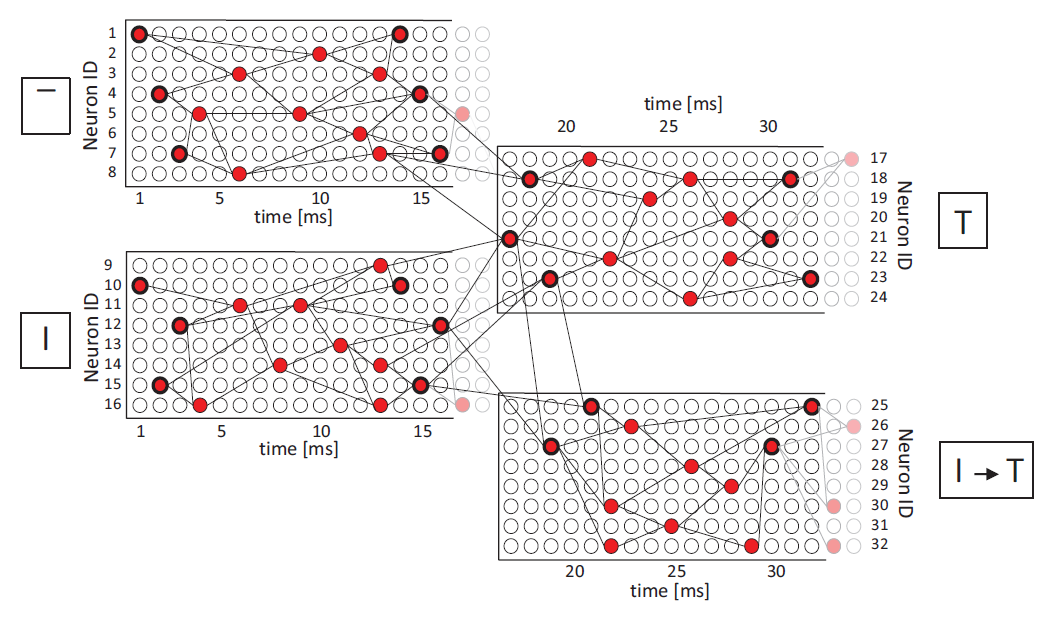
\includegraphics[width=1.0\linewidth]{poly-group-bind.png}
		\caption[NS]{
			نمود رخدادن مثال ذکر‌شده در شکل \ref{fig:eguchi-binding}  از \gls{binding} در گروه‌های چند‌زمانی \cite{EGUCHI2018a}.
		}
		\label{fig:eguchi-binding-group}
	\end{figure}
	
	\section{ستون‌های قشری، واحد‌های مستقل محاسباتی}
	\label{section:hawkins}
	
	هاوکینز در کتابی \cite{Hawkins2021-rq} که حاصل مجموعه تحقیقات‌ وی و همکارانش
	\cite{Hawkins2016, Hawkins2017, Lewis2019}
	بود، با فرض این‌که ستون‌های قشری در سراسر نوقشر ساختار‌های مشابهی دارند و عملکرد آن‌ها صرفاً به دلیل تفاوت ورودی‌های آن‌ها است \cite{Mountcastle1978}، یک مدل محاسباتی برای حل مسئله‌ی \gls{binding} پیشنهاد داد. با فرض این‌که هر ستون قشری مسئولیت درک مفهومی را بر عهده دارد و با علم بر این‌که می‌تواند بین لایه‌های متناظر برخی ستون‌های قشری با فاصله‌ی مکانی بالا، \gls{longdistancecon}\LTRfootnote{Long-distance connections} شکل بگیرد، این فرضیه را مطرح کرد که این اتصالات از راه دور می‌توانند به‌وجود‌آورنده‌ی نوعی سازوکار رای‌گیری باشند که  موجب شکل‌گیری \gls{binding} در مغز می‌شود.
	
	برای انجام رای گیری، هر ستون قشری با توجه به داده‌های ورودی خود، در صورت حضور مجموعه‌ای از مفاهیم فعال خواهد بود و برای دیگر مفاهیم فعالیت کمتری خواهد داشت. با استفاده از اتصالات از راه دور، هر ستون قشری فعالیت و عدم فعالیت خود را به دیگر ستون‌های قشری مخابره می‌کند و در ستون‌های قشری دیگر، مفاهیم محتمل‌تر، مفاهیم با احتمال پایین‌تر را خنثی کرده و  از روی فعالیت چندین ستون قشری یک مفهوم جامع‌تر حاصل از فعالیت دیگر ستون‌ها شکل می‌گیرد. پیش از این نیز تحقیقاتی این احتمال را مطرح کرده‌بودند که انشعابات مختلف دندریتی می‌توانند به عنوان تشخیص‌دهنده‌های الگو‌های مستقل از هم عمل کنند \cite{POIRAZI2003989, Polsky2004} که در این پژوهش نیز این مورد فرض شده که این الگو‌های مستقل در‌واقع بیانگر احتمالات مختلف هستند و با توجه به این‌که بیشتر جمعیت نورون‌های تحریکی را در نوقشر، نورون‌های هرمی تشکیل می‌دهند، مخابره‌کردن این پیام‌های از راه دور درواقع بر عهده‌ی دندریت‌های رأسی و آن دسته از دندریت‌های قاعده‌ای‌ است که فاصله‌ی بیشتری از بدنه‌ی نورون دارند؛ به این صورت که افزایش اختلاف پتانسیل از طریق این دسته‌ از دندریت‌ها باعث نزدیک‌تر شدن نورون به \gls{thresh}‌ی ضربه می‌شوند ولی باعث ضربه نمی‌شوند و صرفاً شرایط را برای رسیدن به آستانه‌ی ضربه از طریق فعالیت دندریت‌های نزدیک‌تر به مبدأ، فراهم می‌کنند.
	
	مدل پیشنهادی آن‌ها (شکل \ref{fig:hawkins2017}) برای ستون‌های قشری، یک مدل دو‌لایه‌ است که ورودی ستون قشری وارد یکی از لایه‌ها شده و از آن لایه پس از پردازش به لایه‌ی دیگر منتقل شده و سپس از لایه‌‌ی دوم از طریق اتصالات از راه دور به لا‌‌یه‌های دوم دیگر ستون‌های قشری منتقل می‌شوند. همچنین آن‌ها مجموعه‌ای از اتصالات پس‌خور\LTRfootnote{F‌‌‌eedback Connections} را نیز از لایه‌ی دوم به لا‌یه‌ی اول تعریف کردند که وظیفه‌ی آن‌ها ارائه‌ی یک پیش‌نمایش از مفهوم‌ شکل‌گرفته در لايه‌ی دوم است که باعث تعادل و هماهنگی بین دو‌لایه‌ می‌شود. در مطالعه‌ی صورت‌گرفته توسط آن‌ها\cite{Hawkins2017} مفهوم مورد بررسی، درک موقعیت‌های مکانی از روی داده‌های مربوط به حس لامسه بوده‌ و انتظار آن‌ها شکل‌گیری یک فعالیت پایدار متناظر با مکان مورد لمس در لایه‌ی دوم، بدون لحاظ‌شدن حالت خود شئ (زاویه و جهت) بوده‌است. 
	
	\begin{figure}[]
		\centering
		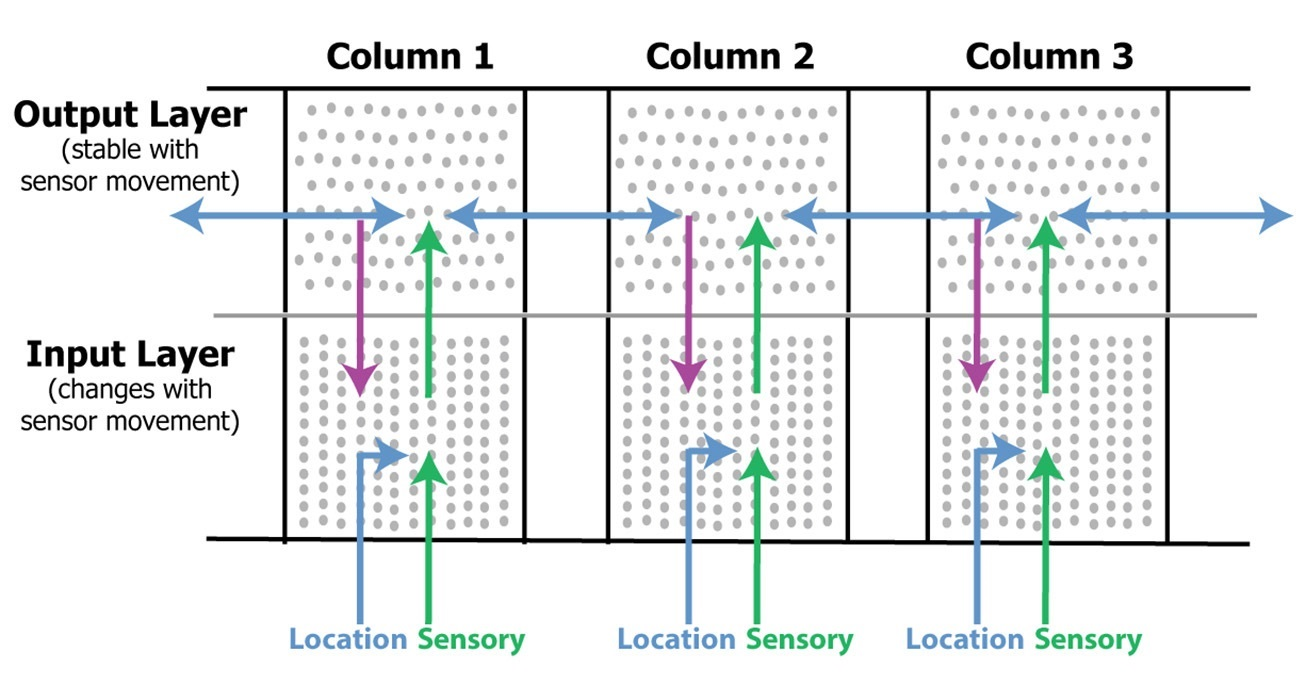
\includegraphics[width=1.0\linewidth]{hawkins2017.jpg}
		\caption[NS]{
			مدل پیشنهادی در مطالعه‌ی صورت‌گرفته \cite{Hawkins2017} برای درک موقعیت‌های مکانی با استفاده از داده‌های مربوط به لامسه و حرکت انگشت‌ها.
		}
		\label{fig:hawkins2017} 
	\end{figure}

در شبکه‌ی ارائه‌شده توسط آن‌ها، برای شبیه‌سازی نورون‌ها از مدل نورونی  \lr{HTM} (که به عبارت «\gls{htm}\LTRfootnote{Hierarchical Temporal Memory}» دلالت دارد) استفاده شده‌است \cite{HTM2011}. همان‌طور که از عنوان این مدل نورونی مشخص است، \lr{HTM}‌ها نورون‌هایی حافظه‌محور هستند. آن‌ها روی مجموعه‌ی بسیار بزرگی از داده‌های زمانی آموزش داده شده‌اند و مجموعه‌ی بزرگی از دنباله‌ها و الگوی‌های رفتاری را در خود ذخیره می‌کنند. حافظه‌ی این دسته از نورون‌ها دارای سازماندهی سلسله‌مراتبی بوده و ذاتاً مبتنی بر زمان است.

یکی دیگر از ویژگی‌های این مدل نورونی آن است که در ورودی‌های آن تفاوت بین دندریت‌های رأسی و قاعده‌ای در نظر گرفته‌‌ شده‌است و تلاش شده تا رفتار نورون‌های هرمی به صورت دقیق‌تر و نزدیک‌تر به حالت زیستی آن مدل‌سازی شود. هرچند با وجود این‌که این مدل نسبت به شبکه‌های عصبی مصنوعی کلاسیک، شباهت بیشتری به نورون‌های زیستی دارد، ولی به اندازه‌ی مدل‌های نورونی ضربه‌ای مشابه با نورون‌های زیستی نمی‌باشد.

\section{استفاده‌ از مدل مبتنی بر ستون قشری در شبکه‌های عصبی}
در پژوهشی دیگر، فردریک الکساندر\LTRfootnote{Frédéric Alexandre} و همکارانش یک واحد محاسباتی  بسیار ساده‌ی الهام گرفته‌شده از ستون‌های قشری را برای استفاده در شبکه‌های عصبی ارائه کردند \cite{Alexandre1991}. آن‌ها از این واحد در یک شبکه‌ی عصبی چند لایه برای \gls{patternrec} استفاده کردند.
آن‌ها برای این واحد محاسباتی، \gls{af}\LTRfootnote{Activation Function} و قانون یادگیری مختص به خود را ارائه دادند. برای مدل‌سازی یک ستون‌قشری از \gls{tt}\LTRfootnote{Truth Table} استفاده کرده و حالت‌های مختلف خروجی ستون‌های قشری را به نسبت ورودی‌های مختلف در آن لیست نموده و  یک تابع فعال‌ساز هماهنگ با آن داده‌ها را ارائه دادند. 
	قانون یادگیری‌ ارائه‌شده توسط آن‌ها، یک یادگیری بر اساس قانون یادگیری هب است. به این صورت که در ابتدا تمام مقادیر به صورت تصادفی توزیع شده‌اند و در روند یادگیری بر اساس هم‌زمانی و یا عدم هم‌زمانی فعالیت دو مفهوم متوالی، احتمال فعال شدن مفهوم ثانویه با فعالیت مفهوم اولیه افزایش یا کاهش می‌یابد.
آن‌ها از این مدل برای تشخیص گفتار و تصویر استفاده کردند و در برخی از حالت‌ها این مدل عملکرد بسیار مناسبی را از خود نشان داد ولی مدل آن‌ها به دلیل ساده‌سازی بیش از حد با رفتار نورون‌های زیستی فاصله‌ی بسیار زیادی دارد.


\section{استفاده از \gls{gnn} برای تشکیل انقیاد}
در پژوهشی، صادقی و همکارانش با استفاده از یک معماری \gls{enc-dec}ی\LTRfootnote{Encoder-decoder} مولد\LTRfootnote{Generative} که نگاه خود را تطبیق می‌دهد و بین ویژگی‌ها با استفاده از \gls{hindsight-reasoning}\LTRfootnote{Hindsight Reasoning} انقیاد ایجاد می‌کند، الگو‌های حرکتی زیستی را مدل‌سازی کرده‌اند \cite{Sadeghi2021}.
آن‌ها در ابتدا مدلی را آموزش دادند که حرکت‌های زیستی پویا یا دیگر الگوی‌های حرکتی دارای‌ هارمونی را یاد بگیرد. سپس داده‌های ورودی را کمی درهم‌ریخته‌ کرده و خطای پیش‌بینی را بر روی یک ماتریس انقیاد، که یک لایه‌ی عصبی و نمایانگر انقیاد ویژگی‌ها است، ذخیره کردند. علاوه‌ بر این، آن‌ها خطا را به سمت نورون‌های نماینده‌ی دیدگاه مدل نشر دادند که وظیفه‌ی این نورون‌ها ترجمه‌ی مقادیر ورودی به \gls{reference-frames}\LTRfootnote{Reference Frames} (یک دستگاه مختصاتی که در آن مکان، جهت و دیگر ویژگی‌های یک پدیده سنجیده می‌شود) است.

در مدل ارائه‌شده توسط آن‌ها، شبکه‌ی عصبی روی ویژگی $i$ام تصویر، تبدیل‌های انتقال و چرخش اعمال می‌شود و در گام بعدی، آن ویژگی‌ها به جمعیت‌های نورونی کد می‌شوند. ماتریس انقیاد، ویژگی $i$ام را به ورودی $j$ام رمزگذار متناظر می‌کند. رمزگذار-رمزگشا الگوی مشاهده‌شده را بازسازی می‌کند و از میزان خطای حاصل‌شده برای تنظیم‌کردن پارامتر‌های ماتریس‌های انقیاد، چرخش و انتقال  از طریق استنتاج پس‌نگر استفاده می‌شود (تصویر \ref{fig:gnn}).

\begin{figure}[]
	\centering
	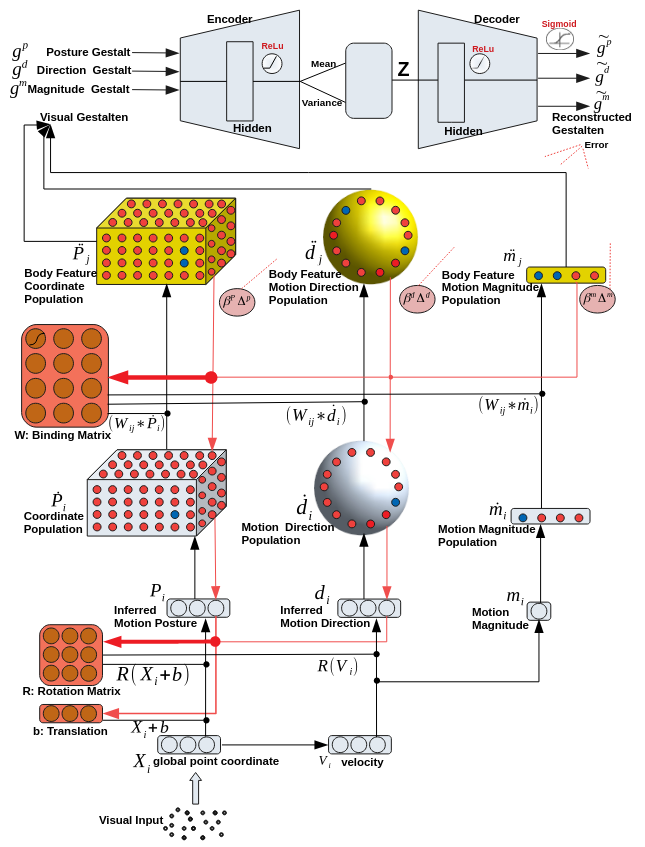
\includegraphics[width=0.8\linewidth]{gnn.png}
	\caption[NS]{
		مدل رمزگذار-رمزگشای مولد ارائه‌شده در  \cite{Sadeghi2021}.
	}
	\label{fig:gnn}
\end{figure}

ارزیابی‌ها نشان دادند که این فرآیند استنتاج، انقیاد را برای الگو‌های شناخته‌شده‌ی حرکتی زیستی به وجود می‌آورد و یک درک گشتالتی\LTRfootnote{Gestalt}  تشکیل می‌دهد؛ یعنی به عبارتی در مدل ارائه‌شده یک مفهوم از روی ورودی شکل می‌گیرد که در خود اطلاعاتی بیشتر از آنچه صرفا در یک ورودی مشاهده کرده‌است، گنجانده. تشکیل این درک گشتالتی خود یک بیان ضعیف از شکل گرفتن انقیاد در این مدل است.
	همچنین آن‌ها این احتمال را مطرح کردند که احتمالا مدل ارائه‌شده توسط آن‌ها باید بتواند برای انقیاد بین مفاهیم \gls{gestalt}ی در دیگر حوزه‌ها نیز موثر باشد.
	
	
	
	\chapter{مدل پیشنهادی، آزمایش‌ها و نتایج}
	
	با توجه به مدل ارائه‌شده توسط‌ هاوکینز و همکارانش و مشخص‌بودن اهمیت ستون‌های قشری در شناخت و شکل‌گیری انقیاد، استفاده از این ساختار در طراحی آزمایشی به منظور مدل‌سازی و بررسی انقیاد در مغز می‌تواند تصمیم درستی باشد. همچنین با توجه به این‌که مدل مذکور یک مدل الهام گرفته‌شده از ساختار زیستی مغز و \gls{snn} نیز، مشابه با آن، روشی الهام‌گرفته از ساختار طبیعی مغز است، می‌تواند گزینه‌ی مناسبی برای مدل‌سازی نورون‌ها باشد. از این رو قصد داریم در ادامه‌ی این فصل مدلی مبتنی بر \gls{snn} با الهام از ساختار ستون‌های قشری طراحی کرده و شکل‌گیری انقیاد در آن را بررسی کنیم و در نهایت نیز نتایج حاصل از این تحقیق را بیان خواهیم کرد.
	
	\section{مدل پیشنهادی}
	
	مدل ارائه‌شده در این بخش شامل یک شبکه‌ی متشکل از سه ستون قشری و ارتباطات بین آن‌ها است. معماری این شبکه مطابق با ساختار مغز موجودات زنده می‌باشد که در آن اطلاعات چند ستون قشری، پس از پردازش، در ستون‌های قشری دیگر تجمیع می‌شوند و مفاهیم پیچیده تر را تشکیل می‌دهند. همچنین دو جمعیت با فعالیت از پیش مشخص‌شده نیز برای وارد کردن اطلاعات ورودی به شبکه مورد استفاده قرار می‌گیرند. فعالیت روی جمعیت‌های ورودی به دو وضعیت تقسیم شده‌است که در هر یک نیمی از نورون‌ها نسبت به دیگر نورون‌ها فعالیت بیشتری دارند. بین این دو مجموعه از نورون‌های فعال به ازای هر وضعیت هیچ اشتراکی وجود ندارد؛ به عبارتی دیگر، هر جمعیت از ورودی‌ها در هر زمان یک الگوی فعالیت از دو الگوی فعالیت ممکن را دارند. دو جمعیت ورودی همواره از نظر الگوی فعالیت مشابه یکدیگر هستند و زمان تغییر الگوی فعالیت نیز هم‌زمان با یکدیگر الگو‌های فعالیتشان تغییر می‌کند. این دو جمعیت ورودی نمایانگر دو ورودی حسی هستند که با تغییر محیط عامل، الگوی فعالیت آن‌ها نیز تغییر می‌کند. برای مثال اگر فرض کنیم عامل در محیطی قرار دارد که دو ورودی حسی (مثل شنوایی و لامسه) به دلیل حضور عامل در محیط، توسط عامل دریافت می‌شود، هر جمعیت متناظر با یکی از ورودی‌ها خواهد بود که هر دو هم‌زمان یا الگوی متناظر با حس کردن موجودیت اول را نشان‌ می‌دهند و یا هر دو هم‌زمان الگوی متناظر با حس‌کردن موجودیت دوم را نشان می‌دهند.
	
	هر یک از این جمعیت‌های ورودی اطلاعات خود‌ را به صورت مستقیم به یکی از ستون‌های قشری منتقل می‌کنند و هریک از این ستون‌های قشری نیز با یک ستون قشری سوم در ارتباط هستند که مسئول یک‌پارچه کردن مفهوم درک‌شده توسط دو ستون قشری است. ارتباط بین دو ستون قشری متصل به ورودی با ستون قشری سوم هم به صورت پیش‌خور و هم به صورت پس‌خور می‌باشد. 
	اتصالات بین دو ستون قشری، به شکلی که در بخش \ref{subsection:pyramidal_neurons} مطرح شد و در پژوهش صورت گرفته در بخش \ref{section:hawkins} از آن‌ها برای پیاده سازی یک سازوکار رأی گیری استفاده شد، نماینده‌ی اتصالات از راه دور هستند.
	انتظار می‌رود مجموعه‌ی سه ستون قشری، که جزئیات ساختار ارتباطی آن‌ها متعاقبا بیان خواهد شد، به یک درک واحد از موجودیت حاضر در محیط برسند و عملا انقیاد در آن مشخص باشد.
	
	
	\subsection{الگوی فعالیت جمعیت‌های ورودی}
	
	همان‌طور که پیش‌تر مطرح شد، جمعیت‌های ورودی در طول زمان دو الگوی فعالیت متفاوت را دارند که در هر‌ یک فعالیت نیمی از نورون‌ها نسبت به نیم دیگر نورون‌ها بیشتر است. هر الگو به مدت زمانی از پیش تعیین شده و ثابت نمایش داده می‌شود. در طول این بازه‌ی زمانی هر یک از نورون‌ها به صورت تصادفی با یک احتمال از پیش تعیین‌شده فعال می‌شود که احتمال فعالیت نورون‌های متناظر با الگوی در حال نمایش بسیار بیشتر از فعالیت دیگر نورون‌ها است. همچنین در انتهای هر الگو برای زمان از پیش تعیین‌شده‌ای فعالیت تمام نورون‌ها با احتمالی مشابه رخ می‌دهد  و عملا هیچ یک از دو الگوی از پیش تعیین‌شده در آن بازه قابل رویت نیست. این زمان استراحت برای این منظور در نظر گرفته شده‌است که فعالیت‌های ناشی از نمایش الگوی قبلی کاهش یافته یا از بین برود و تأثیری روی پردازش‌های مربوط به الگوی جدید نداشته باشد. میزان فعالیت نورون‌های در حال استراحت و نورون‌هایی که متناظر با الگوی در حال نمایش نیستند در هر بازه‌ی متناظر با یک الگو دارای خطای متفاوتی با بازه‌ی قبلی است.	
	در طول زمان، تعیین این موضوع که کدام الگو نمایش داده شود به صورت تصادفی و با احتمال یکسان اتفاق می‌افتد. \gls{rasterplot}\LTRfootnote{Raster Plot} مربوط به یک جمعیت ورودی در یک بازه‌ی زمانی در شکل \ref{fig:input-range} قابل رویت است.
	
\begin{figure}[]
	\centering
	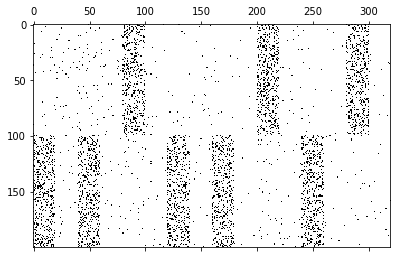
\includegraphics[width=1.0\linewidth]{input-range.png}
	\caption[NS]{
		یک نمونه \gls{rasterplot} مربوط به فعالیت یک جمعیت با ۲۰۰ نورون برای ۳۲۰ واحد زمان که هر الگو برای مدت ۲۰ واحد زمان فعال است و پس از آن برای ۲۰ واحد زمان هیچ الگویی نمایش داده نمی‌شود.
	}
	\label{fig:input-range} 
\end{figure}
	
	\subsection{مدل‌سازی ستون‌های قشری}
	
	برای سادگی در مدل‌سازی، با الگوگیری از پژوهش مطرح‌شده در مقاله‌ی \cite{Hawkins2017}  که در بخش \ref{section:hawkins} به آن پرداخته‌شد، ستون‌های قشری به صورت ساختارهایی دو‌لایه که یک لایه به عنوان لایه‌ی ۴ و لایه‌ی دیگر نیز به عنوان لایه‌‌های ۲ و ۳ (که به صورت ۲/۳ نمایش می‌دهیم) در نوقشر در نظر گرفته‌شده‌اند. در هر یک از لایه‌های ستون‌های قشری دو جمعیت برای بازنمایی دو دسته‌ از نورون‌های فعال برای دو الگوی فعالیت ممکن در نظر گرفته‌شده‌است. بین هر دو جمعیت حاضر در هر لایه یک اتصال مهاری وجود دارد؛ به این صورت که ضربه‌زدن هر نورون باعث یک اثر مهاری روی مجموعه‌ای از نورون‌ها در جمعیت دیگر می‌شود که وجود این اتصال در عمل نقش حضور \gls{inh} را برای ما ایفا می‌کند.
	
	در این مدل جریان اطلاعات از لایه‌ی ۴ به سمت لایه‌ی‌ ۲/۳ است که یک حالت ساده‌شده از اتصالات واقعی بین این بخش‌ها در مغز است و تلاش می‌شود تا در لایه‌ی ۲/۳ یک بازنمایی پایدار‌تر نسبت به لایه‌ی ۴ شکل بگیرد. از این رو یک \gls{poolingcon}\LTRfootnote{Pooling} هر جمعیت لایه‌ی ۴ را به جمعیت متناظر خود در لایه‌ی ۲/۳ متصل می‌کند؛ به این صورت که هر نورون در لایه‌ی ۲/۳ دقیقاً از تعداد مشخصی از نورون‌های لایه‌ی ۴ ورودی دریافت می‌کند و هر نورون در لایه‌ی ۴ تنها به یک نورون در لایه‌ی ۲/۳ متصل است. همچنین وزن این اتصالات به گونه‌ای است که فعالیت حتی یک نورون پیش‌سیناپسی نیز در صورت عدم وجود هیچ‌گونه اثر مهاری، باعث گذر از آستانه و شکل‌گرفتن ضربه در لایه‌ی ۲/۳ می‌شود. 
	
	همچنین در این مدل مجموعه‌ای از اتصالات پس‌خور\LTRfootnote{Backward Connections} نیز در نظر گرفته شده‌است که مشابه با آنچه در بخش \ref{subsection:pyramidal_neurons} مطرح شد، نقش اتصالاتی را بازی می‌کنند که وظیفه‌ی آماده‌کردن نورون‌های پس‌سیناپسی برای ضربه‌زدن را دارند و وزن این دسته از اتصالات مشخص کننده‌ی میزان نزدیک شدن اختلاف پتانسیل نورون پس‌سیناپسی به آستانه است؛ به عبارت دیگر، نورون‌های پس‌سیناپسی را به آستانه‌ی ضربه نزدیک می‌کنند ولی باعث فعال شدن آن‌ها نمی‌شوند. همچنین دسته‌ی دیگری از اتصالات پس‌خور نیز تعریف شده‌اند که مشابه مورد قبل هستند ولی نقش مهاری دارند و با فعال شدن نورون‌های پیش‌سیناپسی، آن دسته از اتصالات به همان نسبت اختلاف پتانسیل را به میزان اختلاف پتانسیل حالت استراحت نورون نزدیک‌تر می‌کنند.
		شمای کلی مدل پیشنهادی برای هر ستون قشری در شکل \ref{fig:model_cc} قابل مشاهده است. 
	
	\begin{figure}[]
		\centering
		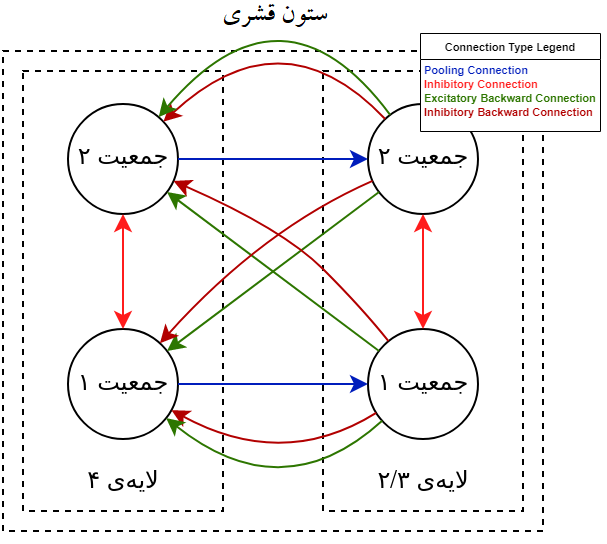
\includegraphics[width=0.9\linewidth]{model_cc.png}
		\caption[NS]{
			شمای کلی ستون قشری که در آن جمعیت‌ها و اتصالات بین آن‌ها مشخص شده‌اند. جهت پیکان‌ها مشخص‌کننده‌ی جمعیت پس‌سیناپسی و رنگ پیکان‌ها مشخص‌کننده‌ی نوع اتصالات است. پیکان آبی نمایان‌گر اتصال ادغام، قرمز روشن نمایان‌گر اتصال مهاری، سبز نمایان‌گر اتصالات پس‌خور تحریکی و  اتصالات با رنگ قرمز تیره مشخص‌کننده‌ی اتصالات پس‌خور مهاری هستند.
		}
		\label{fig:model_cc} 
	\end{figure}
	
	
	\subsection{\gls{feedforwardcon} بین ستون‌های قشری و جمعیت‌های ورودی}
	
	دو ستون قشری‌ که جمعیت‌های ورودی به لایه‌ی ۴ آن‌ها متصل شده‌اند، باید داده را به ستون قشری دیگر (که پس از این با نام «ستون قشری سوم» به آن اشاره می‌کنیم) منتقل کنند تا اطلاعات در آنجا تجمیع شوند و یک درک واحد از ورودی دو ستون قشری در آن‌جا شکل بگیرد. برای این منظور لایه‌ی ۲/۳ این دو ستون قشری با یک اتصال تحریکی به لایه ۴ ستون قشری سوم متصل می‌شود (شکل \ref{fig:model_overall}). به عبارتی هرکدام از جمعیت‌های نورونی موجود در لایه‌ی ۲/۳ هر کدام از ستون‌های قشری اول و دوم، یک اتصال تحریکی به هر‌ یک از جمعیت‌های نورونی لایه‌ی ۴ ستون قشری سوم دارند. 
	
	همچنین از جمعیت‌های ورودی نیز یک اتصال تحریکی به جمعیت‌های حاضر در لایه‌ی ۴ ستون‌های قشری اول و دوم در نظر گرفته‌شده تا فعالیت ورودی‌ها به ستون‌های قشری منتقل شود.
	
	\subsection{اتصالات پس‌خور بین ستون‌های قشری}
	
	مشابه اتصالات پس‌خوری که در داخل هر ستون قشری تعریف شده‌بودند، اتصالاتی بین جمعیت‌های دو ستون قشری نیز تعریف می‌شوند که نقش اتصالات از راه دور موجود در مغز را برای ما ایفا می‌کنند. ساختار این اتصالات به این صورت است که اتصالات از لایه‌ی ۲/۳ ستون قشری سوم به لایه‌های ۲/۳ ستون‌های قشری اول و دوم هم اتصالات پس‌خور تحریکی و هم اتصالات پس‌خور مهاری وجود دارند و سازوکار نوع تحریکی این اتصالات پس‌خور مشابه با اتصالات پس‌خوری که در داخل ستون‌های قشری تعریف شده‌بودند، باعث کاهش فاصله‌ی اختلاف پتانسیل نورون‌های پس‌سیناپسی با آستانه‌ی ضربه می‌شوند ولی مستقلا موجب ضربه نمی‌شوند. نوع مهاری این اتصالات پس‌خور نیز اختلاف پتانسیل نورون‌های پس‌سیناپسی را به اختلاف پتانسیل استراحت نزدیکتر می‌کنند. 
	
	شمای کلی مدل پیشنهاد شده در شکل \ref{fig:model_overall} قابل رؤیت است.
	
	\begin{figure}[]
		\centering
		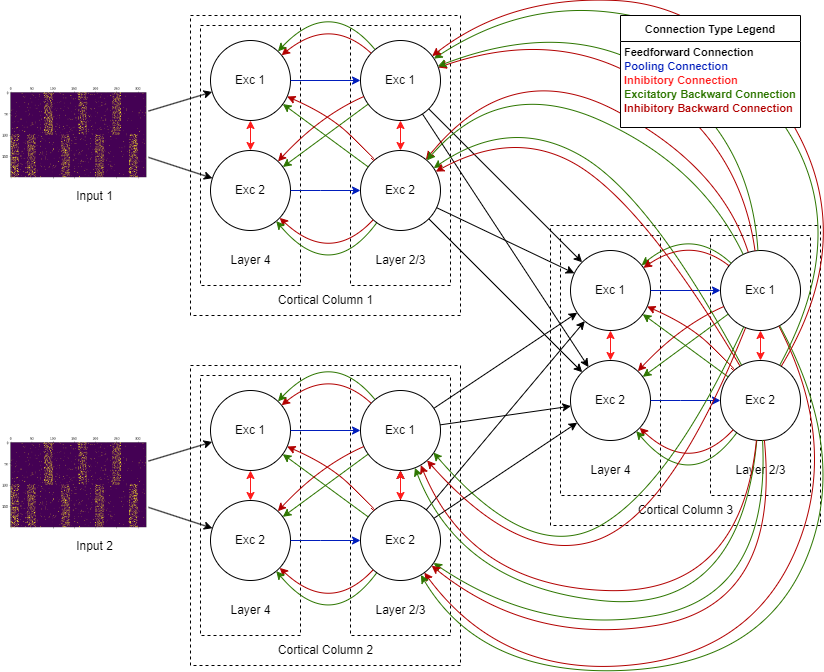
\includegraphics[width=1.0\linewidth]{model_overall.png}
		\caption[NS]{
			مدل پیشنهادی که در آن تمام جمعیت‌ها و اتصالات بین آن‌ها مشخص شده‌است. همچنین رنگ اتصالات نیز مشابه با رنگ اتصالات تعریف‌شده در شکل \ref{fig:model_cc} می‌باشد.
		}
		\label{fig:model_overall} 
	\end{figure}

	\subsection{وزن‌های اولیه و انعطاف‌پذیری نورونی}
	نرخ اتصالات بین هر دو جمعیت در مدل به صورت از پیش تعریف‌شده و ثابت می‌باشد. به این صورت که تعدادی از اتصالات بین دو جمعیت در ابتدای مدل‌سازی به صورت تصادفی با احتمال از پیش تعیین‌شده، انتخاب و کاملاً حذف می‌شوند که برای این منظور وزن سیناپسی‌ آن‌ها برای تمام طول شبیه‌سازی صفر در نظر گرفته می‌شود.
	
	برای مقداردهی اولیه‌ی وزن‌های تمام اتصالات، بجز \gls{feedbackcon}، از توزیع یکنواخت در بازه‌ی مشخص‌شده برای هر جمعیت و برای مقداردهی اولیه‌ی وزن‌های اتصالات پس‌خور نیز از توزیع بتا\LTRfootnote{Beta Distribution} استفاده شده‌است (شکل \ref{fig:beta}). همان‌طور که پیش‌تر نیز اشاره شده‌بود سازوکار اتصالات پس‌خور به گونه‌ای است که وزن آن‌ها بیانگر میزان تأثیرگذاری آن‌ها در اختلاف پتانسیل نورون‌های پس‌سیناپسی است و به همین دلیل مقادیر همواره در بازه‌ی صفر و یک هستند.
	
	\begin{figure}[]
		\centering
		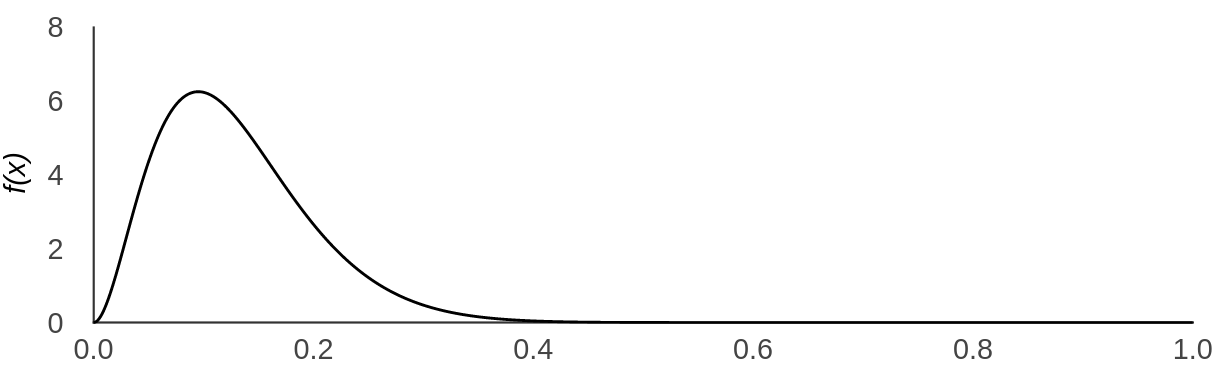
\includegraphics[width=0.8\linewidth]{beta-3-20.png}
		\caption[NS]{
			یک نمونه توزیع بتا با پارامتر‌های $\alpha=3$ و $\beta=20$.
		}
		\label{fig:beta} 
	\end{figure}
	
	همچنین در مدل ارائه‌شده اتصالات متنوعی بین جمعیت‌های مختلف حاضر در مدل به کار گرفته شده‌اند و روی هر یک از آن‌ها نیز می‌توان یک سازوکار برای انعطاف‌پذیری نورونی و تغییرات وزن اتصالات در طول زمان تعریف کرد. لازم به ذکر است که برای مجموعه‌ی اتصالات مهاری بین جمعیت‌های یک لایه از ستون قشری، انعطاف‌پذیری نورونی مشخص نشده و وزن اتصالاتشان در تمام طول شبیه‌سازی ثابت است. تمام قوانین یادگیری مورد استفاده، قوانین یادگیری تقویتی هستند که به دلیل ساختار ورودی‌ها که الگوی رفتاری جمعیت‌های ورودی برای بازه‌هایی با طول زمان مشخص ثابت هستند، شخصی سازی شده‌اند؛ به این صورت که برخلاف رویه‌ی مطرح‌شده در بخش \ref{section:reward-in-brain}، میزان دوپامین نه در هر لحظه، بلکه در انتهای بازه‌ی نمایش هر الگو محاسبه می‌گردد و در طول بازه‌ی نمایش یک الگو در ورودی، هیچ تغییری توسط قوانین یادگیری روی وزن‌های اتصالات اعمال نمی‌شود و تمام این تغییرات تجمیع شده و  با توجه به میزان دوپامین محاسبه‌شده در انتهای هر بازه به صورت یک‌جا روی اتصالات اعمال می‌شوند. میزان تغییرات وزن در زمان $t$ در فرمول \ref{eq:seasonal} مشخص شده‌است که در آن $|I|$ طول بازه‌ی نمایش هر الگوی ورودی و $STDP(t')$ نیز میزان تغییرات وزن در صورت اعمال انعطاف‌پذیری وابسته به زمان ضربه در زمان $t'$ است.
	
	\begin{align}
		\Delta w_t =
		\begin{cases}
			d \times \sum_{t'=t-\left | I \right |+1}^{t} STDP(t') & \text{if}\,~t\bmod\left | I \right | = 0\\
			0 & \text{otherwise.}
		\end{cases}  
		\label{eq:seasonal}
	\end{align}
	
	میزان دوپامین برای پاداش و تنبیه نیز در هر لحظه بر اساس مقایسه‌ی میزان فعالیت (تعداد ضربه‌ها در طول بازه‌ی نمایش الگو) جمعیت‌های لایه‌ی ۲/۳ ستون قشری سوم محاسبه می‌گردد. به این صورت که هر یک از دو الگوی فعالیت که نورون‌های ورودی به خود می‌گیرند، با یکی از دو جمعیت این لایه متناظر می‌شود و در صورتی که جمعیت متناظر با الگوی در حال نمایش فعالیت بیشتری نسبت به جمعیت دیگر داشته باشد، پاداش و در غیر این صورت تنبیه برای مدل لحاظ می‌شود. همچنین میزان شدت پاداش و تنبیه نیز بر اساس میزان اختلاف فعالیت این دو جمعیت بر اساس رابطه‌ی زیر تعیین می‌گردد: 
	
	\begin{subequations}
	\begin{align}
		g &= \frac{| A(pop_1) - A(pop_2) |}{|pop|} \\ 
		d &=
		\begin{cases}
			1 + g & win \,~\text{and}~\, g > 0.3\\
			-0.1 + g & win \,~\text{and}~\, g \le 0.3\\
			-1 - g & \neg win
		\end{cases}  
		\label{eq:reward-calc-2}
	\end{align}
\end{subequations}

در این رابطه $A(pop_x)$ میزان فعالیت جمعیت $x$، $|pop|$ تعداد نورون‌های لایه‌ی ۲/۳ و $win$ نیز برنده شدن جمعیت صحیح را مشخص می‌کند؛ به این صورت که مقدار $win$ تنها در صورتی صحیح خواهد بود که فعالیت جمعیت متناظر با الگوی اول بیشتر باشد و جمعیت نمایش داده شده در ورودی، الگوی اول باشد، و یا این‌که فعالیت جمعیت متناظر با الگوی دوم بیشتر باشد و جمعیت نمایش داده شده در ورودی نیز الگوی دوم باشد. رابطه‌ی \ref{eq:reward-calc-2} از سه ضابطه تشکیل شده است که به ترتیب مربوط به این شرایط هستند:
\begin{enumerate}
	\item جمعیت صحیح، با اختلاف مناسبی در میزان فعالیت جمعیت‌ها، برنده شده است و پاداش داده می‌شود.
	\item جمعیت صحیح با اختلاف بسیار کمی برنده شده و با توجه به میزان این اختلاف ممکن است مقدار کمی پاداش یا تنبیه برای مدل درنظر گرفته شود.
	\item  جمعیت صحیح بازنده شده و مدل تنبیه می‌شود.
\end{enumerate} 
	

	\subsection{ابزار‌های پیاده‌سازی}
	
	پیاده‌سازی‌های مربوط به مدل ارائه‌شده با زبان برنامه‌نویسی پایتون و در بستر چارچوب\LTRfootnote{Framework} نرم‌افزاری بایندزنت\LTRfootnote{Bindsnet}، که خود برپایه‌ی چارچوب پای‌تورچ\LTRfootnote{PyTorch} توسعه داده‌شده‌، انجام شده‌است. از جمله ویژگی‌های مورد نظر که چارچوب نرم‌افزاری بر اساس آن‌ها انتخاب شده‌است می‌توان به توان پردازش محاسبات تنسوری توسط پردازنده و کارت گرافیک، و از پیش تعریف‌شدن مدل‌های نورونی پایه، همچون مدل نورونی تجمیع و آتش، انعطاف‌پذیری نورونی و محاسبات مربوط به اتصالات بین نورون‌ها، اشاره کرد.
	
	همچنین به دلیل نیاز به مجموعه‌ای از سازوکار‌ها و ساختارهایی که در هیچ یک از چارچوب‌های مورد‌ استفاده از پیش تعریف نشده‌بودند، یک چارچوب نرم‌افزاری بر بستر بایندزنت توسعه داده شده‌ که در عمل مدل‌سازی‌های نهایی بر بستر آن انجام شده‌اند.
	
	\subsection{پارامتر‌های مورد استفاده در آزمایش}
	اجزای مختلف مدل ارائه‌شده پارامتر‌های مختلفی دارند که در نتیجه‌ی نهایی آزمایش تأثیر بسیار مهمی می‌گذارند. مواردی همچون تعداد نورون‌های جمعیت‌های مختلف، نرخ‌های یادگیری، نرخ اتصالات بین جمعیت‌ها و بسیاری موارد دیگر. همچنین با توجه به پیچیدگی مدل و پیچیدگی سیستم حاصل از پیاده‌سازی آن با استفاده از شبکه‌های عصبی ضربه‌ای، تنظیم کردن این پارامتر‌ها به گونه‌ای که شبکه عملکرد مناسبی داشته باشد موضوعی بسیار چالش‌برانگیز است. پارامتر‌های مورد استفاده برای آزمایش در سه جدول \ref{table:parameters-cc-1-2}، \ref{table:parameters-cc-3} و \ref{table:parameters-details} مشخص شده‌اند.

\begin{table}[p]
	\centering
	\resizebox{\textwidth}{!}{
	\begin{tabular}{|rrrl|}
		\hline
		\multicolumn{4}{|c|}{\textbf{ستون‌های قشری اول و دوم}}                                                                                                                                                              \\ \hline
		\multicolumn{1}{|r|}{\multirow{8}{*}{لایه ۴}}                   & \multicolumn{1}{r|}{\multirow{6}{*}{جمعیت‌ها}}                 & \multicolumn{1}{r|}{تعداد نورون‌های هر جمعیت}             & $100$                     \\ \cline{3-4} 
		\multicolumn{1}{|r|}{}                                          & \multicolumn{1}{r|}{}                                          & \multicolumn{1}{r|}{اثر ثابت زمانی\LTRfootnote{Time Constant Trace}} & $6$                       \\ \cline{3-4} 
		\multicolumn{1}{|r|}{}                                          & \multicolumn{1}{r|}{}                                          & \multicolumn{1}{r|}{آستانه‌ی ضربه}                        & $-52$                     \\ \cline{3-4} 
		\multicolumn{1}{|r|}{}                                          & \multicolumn{1}{r|}{}                                          & \multicolumn{1}{r|}{ولتاژ استراحت}                        & $-65$                     \\ \cline{3-4} 
		\multicolumn{1}{|r|}{}                                          & \multicolumn{1}{r|}{}                                          & \multicolumn{1}{r|}{بازه‌ی عدم فعالیت پس از ضربه}         & $3$                       \\ \cline{3-4} 
		\multicolumn{1}{|r|}{}                                          & \multicolumn{1}{r|}{}                                          & \multicolumn{1}{r|}{ثابت زمانی کاهش}                      & $10$                      \\ \cline{2-4} 
		\multicolumn{1}{|r|}{}                                          & \multicolumn{1}{r|}{\multirow{2}{*}{اتصال مهاری بین دو جمعیت}} & \multicolumn{1}{r|}{بازه‌ی وزن}                           & $(-0.4,0)$                \\ \cline{3-4} 
		\multicolumn{1}{|r|}{}                                          & \multicolumn{1}{r|}{}                                          & \multicolumn{1}{r|}{نرخ اتصال}                            & $0.3$                     \\ \hline
		\multicolumn{1}{|r|}{\multirow{8}{*}{\textbf{لایه ۲/۳}}}        & \multicolumn{1}{r|}{\multirow{6}{*}{جمعیت‌ها}}                 & \multicolumn{1}{r|}{تعداد نورون‌های هر جمعیت}             & $32$ \\ \cline{3-4} 
		\multicolumn{1}{|r|}{}                                          & \multicolumn{1}{r|}{}                                          & \multicolumn{1}{r|}{اثر ثابت زمانی} & $10$                      \\ \cline{3-4} 
		\multicolumn{1}{|r|}{}                                          & \multicolumn{1}{r|}{}                                          & \multicolumn{1}{r|}{آستانه‌ی ضربه}                        & $-52$                     \\ \cline{3-4} 
		\multicolumn{1}{|r|}{}                                          & \multicolumn{1}{r|}{}                                          & \multicolumn{1}{r|}{ولتاژ استراحت}                        & $-65$                     \\ \cline{3-4} 
		\multicolumn{1}{|r|}{}                                          & \multicolumn{1}{r|}{}                                          & \multicolumn{1}{r|}{بازه‌ی عدم فعالیت پس از ضربه}         & $3$                       \\ \cline{3-4} 
		\multicolumn{1}{|r|}{}                                          & \multicolumn{1}{r|}{}                                          & \multicolumn{1}{r|}{ثابت زمانی کاهش}                      & $10$                      \\ \cline{2-4} 
		\multicolumn{1}{|r|}{}                                          & \multicolumn{1}{r|}{\multirow{2}{*}{اتصال مهاری بین دو جمعیت}} & \multicolumn{1}{r|}{بازه‌ی وزن}                           & $(-0.4,0)$                \\ \cline{3-4} 
		\multicolumn{1}{|r|}{}                                          & \multicolumn{1}{r|}{}                                          & \multicolumn{1}{r|}{نرخ اتصال}                            & $1.0$                     \\ \hline
		\multicolumn{1}{|r|}{\multirow{3}{*}{اتصال ادغام بین دو لایه}} & \multicolumn{2}{r|}{اندازه‌ی کرنل}                                                                                         & $5$                       \\ \cline{2-4} 
		\multicolumn{1}{|r|}{}                                          & \multicolumn{2}{r|}{وزن اتصال}                                                                                             & $14$                      \\ \cline{2-4} 
		\multicolumn{1}{|r|}{}                                          & \multicolumn{2}{r|}{اندازه‌ی گام}                                                                                          & $3$                       \\ \hline
		\multicolumn{1}{|r|}{\multirow{6}{*}{اتصالات پس‌خور}}        & \multicolumn{2}{r|}{پارامتر‌های توزیع بتا}                                                                                 & $\alpha=3, \beta=40$               \\ \cline{2-4} 
		\multicolumn{1}{|r|}{}                                          & \multicolumn{2}{r|}{نرخ اتصال}                                                                                             & $0.2$                     \\ \cline{2-4} 
		\multicolumn{1}{|r|}{}                                          & \multicolumn{2}{r|}{بازه‌ی وزن}                                                                                            & $(0, 0.95)$               \\ \cline{2-4} 
		\multicolumn{1}{|r|}{}                                          & \multicolumn{2}{r|}{نرخ یادگیری}                                                                                           & $0.003 - 0.008$           \\ \cline{2-4} 
		\multicolumn{1}{|r|}{}                                          & \multicolumn{2}{r|}{وزن کاهش}                                                                                              & $0.00005$                \\ \cline{2-4} 
		\multicolumn{1}{|r|}{}                                          & \multicolumn{2}{r|}{ثابت زمانی}                                                                                            & $6$                       \\ \hline
	\end{tabular}}
\caption{\label{table:parameters-cc-1-2}پارامتر‌های مربوط به ستون‌های قشری اول و دوم}
\end{table}


\begin{table}[p]
	\centering
	\resizebox{\textwidth}{!}{
		\begin{tabular}{|rrrl|}

\hline
\multicolumn{4}{|c|}{\textbf{ستون‌ قشری سوم}}                                                                                                                                                               \\ \hline
\multicolumn{1}{|r|}{\multirow{8}{*}{لایه ۴}}                   & \multicolumn{1}{r|}{\multirow{6}{*}{جمعیت‌ها}}                 & \multicolumn{1}{r|}{تعداد نورون‌های هر جمعیت}     & $100$                     \\ \cline{3-4} 
\multicolumn{1}{|r|}{}                                          & \multicolumn{1}{r|}{}                                          & \multicolumn{1}{r|}{اثر ثابت زمانی}               & $6$                       \\ \cline{3-4} 
\multicolumn{1}{|r|}{}                                          & \multicolumn{1}{r|}{}                                          & \multicolumn{1}{r|}{آستانه‌ی ضربه}                & $-52$                     \\ \cline{3-4} 
\multicolumn{1}{|r|}{}                                          & \multicolumn{1}{r|}{}                                          & \multicolumn{1}{r|}{ولتاژ استراحت}                & $-65$                     \\ \cline{3-4} 
\multicolumn{1}{|r|}{}                                          & \multicolumn{1}{r|}{}                                          & \multicolumn{1}{r|}{بازه‌ی عدم فعالیت پس از ضربه} & $3$                       \\ \cline{3-4} 
\multicolumn{1}{|r|}{}                                          & \multicolumn{1}{r|}{}                                          & \multicolumn{1}{r|}{ثابت زمانی کاهش}              & $10$                      \\ \cline{2-4} 
\multicolumn{1}{|r|}{}                                          & \multicolumn{1}{r|}{\multirow{2}{*}{اتصال مهاری بین دو جمعیت}} & \multicolumn{1}{r|}{بازه‌ی وزن}                   & $(-0.3,0)$                \\ \cline{3-4} 
\multicolumn{1}{|r|}{}                                          & \multicolumn{1}{r|}{}                                          & \multicolumn{1}{r|}{نرخ اتصال}                    & $0.3$                     \\ \hline
\multicolumn{1}{|r|}{\multirow{8}{*}{لایه ۲/۳}}                 & \multicolumn{1}{r|}{\multirow{6}{*}{جمعیت‌ها}}                 & \multicolumn{1}{r|}{تعداد نورون‌های هر جمعیت}     & $32$ \\ \cline{3-4} 
\multicolumn{1}{|r|}{}                                          & \multicolumn{1}{r|}{}                                          & \multicolumn{1}{r|}{اثر ثابت زمانی}               & $10$                      \\ \cline{3-4} 
\multicolumn{1}{|r|}{}                                          & \multicolumn{1}{r|}{}                                          & \multicolumn{1}{r|}{آستانه‌ی ضربه}                & $-52$                     \\ \cline{3-4} 
\multicolumn{1}{|r|}{}                                          & \multicolumn{1}{r|}{}                                          & \multicolumn{1}{r|}{ولتاژ استراحت}                & $-65$                     \\ \cline{3-4} 
\multicolumn{1}{|r|}{}                                          & \multicolumn{1}{r|}{}                                          & \multicolumn{1}{r|}{بازه‌ی عدم فعالیت پس از ضربه} & $3$                       \\ \cline{3-4} 
\multicolumn{1}{|r|}{}                                          & \multicolumn{1}{r|}{}                                          & \multicolumn{1}{r|}{ثابت زمانی کاهش}              & $10$                      \\ \cline{2-4} 
\multicolumn{1}{|r|}{}                                          & \multicolumn{1}{r|}{\multirow{2}{*}{اتصال مهاری بین دو جمعیت}} & \multicolumn{1}{r|}{بازه‌ی وزن}                   & $(-0.3,0)$                \\ \cline{3-4} 
\multicolumn{1}{|r|}{}                                          & \multicolumn{1}{r|}{}                                          & \multicolumn{1}{r|}{نرخ اتصال}                    & $1.0$                     \\ \hline
\multicolumn{1}{|r|}{\multirow{3}{*}{اتصال ادغام بین دو لایه}} & \multicolumn{2}{r|}{اندازه‌ی کرنل}                                                                                 & $5$                       \\ \cline{2-4} 
\multicolumn{1}{|r|}{}                                          & \multicolumn{2}{r|}{وزن اتصال}                                                                                     & $14$                      \\ \cline{2-4} 
\multicolumn{1}{|r|}{}                                          & \multicolumn{2}{r|}{اندازه‌ی گام}                                                                                  & $3$                       \\ \hline
\multicolumn{1}{|r|}{\multirow{6}{*}{اتصالات پس‌خور}}        & \multicolumn{2}{r|}{پارامتر‌های توزیع بتا}                                                                         & $\alpha=3, \beta=80$               \\ \cline{2-4} 
\multicolumn{1}{|r|}{}                                          & \multicolumn{2}{r|}{نرخ اتصال}                                                                                     & $0.2$                     \\ \cline{2-4} 
\multicolumn{1}{|r|}{}                                          & \multicolumn{2}{r|}{بازه‌ی وزن}                                                                                    & $(0, 0.95)$               \\ \cline{2-4} 
\multicolumn{1}{|r|}{}                                          & \multicolumn{2}{r|}{نرخ یادگیری}                                                                                   &    $0.003 - 0.007$        \\ \cline{2-4} 
\multicolumn{1}{|r|}{}                                          & \multicolumn{2}{r|}{وزن کاهش}                                                                                      & $0.00005$                \\ \cline{2-4} 
\multicolumn{1}{|r|}{}                                          & \multicolumn{2}{r|}{ثابت زمانی}                                                                                    & $6$                       \\ \hline
	\end{tabular}}
\caption{\label{table:parameters-cc-3}پارامتر‌های مربوط به ستون قشری سوم}
\end{table}


\begin{table}[p]
\centering
\resizebox{0.95\textwidth}{!}{
	\begin{tabular}{|rrrl|}
		\hline
		\multicolumn{4}{|c|}{\textbf{جمعیت‌های ورودی}}                                                                  \\ \hline
		\multicolumn{3}{|r|}{تعداد نورون‌ها}                                                      & $200$                 \\ \hline
		\multicolumn{3}{|r|}{اثر ثابت زمانی}                                & $6$                   \\ \hline
		\multicolumn{4}{|c|}{\textbf{اتصالات جمعیت ورودی به ستون‌های قشری}}                                          \\ \hline
		\multicolumn{3}{|r|}{بازه‌ی وزن}                                                          & $(0, 0.5)$            \\ \hline
		\multicolumn{3}{|r|}{نرخ یادگیری مثبت}                                                    & $0.01$                \\ \hline
		\multicolumn{3}{|r|}{نرخ یادگیری منفی}                                                    & $0.02$               \\ \hline
		\multicolumn{3}{|r|}{نرخ اتصال}                                                           & $0.3$                 \\ \hline
		\multicolumn{3}{|r|}{ثابت زمانی}                                                          & $6$                   \\ \hline
		\multicolumn{4}{|c|}{\textbf{الگو‌های فعالیت ورودی}}                                                            \\ \hline
		\multicolumn{3}{|r|}{زمان نمایش هر الگو}                                                  & $20$                  \\ \hline
		\multicolumn{3}{|r|}{زمان استراحت (بدون نمایش الگو پس از هر نمایش الگو)}                  & $20$                  \\ \hline
		\multicolumn{3}{|r|}{احتمال فعالیت نورون‌ها در زمان استراحت}                              & $0.01\pm 0.005$        \\ \hline
		\multicolumn{3}{|r|}{احتمال فعالیت نورون‌ها در زمان نمایش الگو}                           & $\sim 0.2$           \\ \hline
		\multicolumn{4}{|c|}{\textbf{اتصالات پس‌خور بین ستون‌های قشری}}                                           \\ \hline
		\multicolumn{3}{|r|}{پارامتر‌های توزیع بتا}                                               & $\alpha=3, \beta=80$           \\ \hline
		\multicolumn{3}{|r|}{نرخ اتصال}                                                           & $0.2$                 \\ \hline
		\multicolumn{3}{|r|}{بازه‌ی وزن}                                                          & $(0, 0.95)$           \\ \hline
		\multicolumn{3}{|r|}{نرخ یادگیری}                                                         & $0.003 - 0.007$       \\ \hline
		\multicolumn{3}{|r|}{وزن کاهش}                                                            & $0.00005$             \\ \hline
		\multicolumn{3}{|r|}{ثابت زمانی}                                                          & $6$                   \\ \hline
		\multicolumn{4}{|c|}{\textbf{زمان‌های آموزش}}                                                                   \\ \hline
		\multicolumn{3}{|r|}{تعداد الگو‌های نمایش داده شده برای آموزش ستون‌های قشری اول و دوم} & $800$                \\ \hline
		\multicolumn{3}{|r|}{تعداد الگو‌های نمایش داده شده در گام اول همراه با اتصالات پس‌خور} & $200$                \\ \hline
		\multicolumn{3}{|r|}{تعداد الگو‌های نمایش داده شده برای آموزش ستون قشری سوم}           & $500$                 \\ \hline
\end{tabular}}
\caption{\label{table:parameters-details}پارامتر‌های جزئی مربوط به مدل مورد استفاده}
\end{table}





	
	\section{روند آموزش مدل پیشنهادی}
	برای رسیدن به نتیجه‌ی نهایی که شکل‌گیری انقیاد در مدل طراحی‌شده‌ است، لازم است تا مدل آموزش داده شود تا وزن‌های سیناپسی متناسب با داده‌های ورودی یادگرفته شوند. 
	فرآیند آموزش مدل شامل سه مرحله‌ی اصلی خواهد بود:
	
	\begin{enumerate}
		\item آموزش ستون قشری متناظر با اولین جمعیت ورودی و اتصالات بین جمعیت ورودی و ستون قشری.
		\item آموزش ستون قشری متناظر با دومین جمعیت ورودی و اتصالات بین جمعیت ورودی و ستون قشری.
		\item آموزش اتصالاتی که در آن‌ها ستون قشری سوم دخیل است با استفاده از دو ستون قشری آموزش داده شده‌ی قبلی.
	\end{enumerate}

	در گام اول برای آموزش ستون‌های قشری متناظر با جمعیت‌های ورودی (دو مرحله‌ی اول آموزش) شبکه‌ای به صورت محدود شامل جمعیت ورودی و ستون قشری متناظر، بدون اتصالات پس‌خور در نظر گرفته می‌شود و برای مدت زمان مشخصی شبکه اجرا می‌شود. با توجه به عدم حضور ستون قشری سوم در این شبکه، میزان دوپامین در این شبکه با سازوکاری مشابه با مدل اصلی توسط لایه ۲/۳ ستون قشری حاضر محاسبه می‌شود. سپس به این شبکه اتصالات پس‌خور همان ستون قشری نیز اضافه شده و مجدداً برای زمانی کوتاه‌تر از زمان اجرای پیشین، یادگیری شبکه در مجاورت ورودی ادامه پیدا می‌کند.
	
	در گام قبلی که ستون‌های قشری اول و دوم آموزش داده شدند، وزن‌های سیناپسی اتصالات آن‌ها پس از آموزش مشخص شده. در گام بعدی از این وزن‌های حاصل شده از آموزش هر‌یک از دو ستون قشری اول و دوم، در مدل اصلی، که شامل ستون قشری سوم نیز می‌باشد، جایگزین می‌شوند و یادگیری روی این دسته از سیناپس‌ها، که خود از آموزش حاصل شده‌اند، متوقف می‌شود. سپس مجدداً شبکه برای مدت زمان مشخصی اجرا می‌شود تا وزن‌های سیناپسی مربوط به اتصالات بین مدل‌های قبلی و ستون قشری سوم نیز آموزش داده شوند.
	

	\section{نتایج}
	پس از این‌که مدل آموزش داده‌ شد، وزن‌های اتصالات بین جمعیت‌ها که در ابتدا به صورت تصادفی توزیع شده بودند، تغییر کرده‌اند. با توجه به این‌که آموزش در دو گام کلی رخداده بود، نتایج این آزمایش نیز در دو بخش مربوط به نتایج آموزش ستون‌های قشری اول و دوم، که ستون‌های متصل به ورودی بودند، و ستون قشری سوم، که حاصل تجمیع اطلاعات دو ستون قشری پیشین بود، گزارش می‌گردد.
	برای سادگی، در این گزارش تنها نتایج مربوط به یک آزمایش بخصوص گزارش شده‌است، ولی فرآیند آموزش و نتایج آن کاملاً تکرار‌پذیر هستند و منحصر به تلاش‌های خاصی نمی‌شوند.
	همچنین در ادامه‌ی فصل به مشخص کردن میزان پیشرفت یادگیری و  گزارش دقت نهایی مدل در تلاش‌ها‌ی مختلف اشاره خواهیم کرد.
	
	\subsection{نتایج آموزش ستون‌های قشری اول و دوم}
	طبیعتا در ابتدای فرآیند آموزش، الگوی رفتاری مدل شکلی تصادفی دارد و بین الگوی نمایش داده شده در جمعیت‌های ورودی و الگوی رفتاری جمعیت‌های لایه‌ی ۲/۳ ستون قشری، هم‌بستگی بسیار کمی وجود دارد. یک نمونه فعالیت جمعیت‌های لایه‌ ۲/۳ ستون قشری در 400 میلی‌ثانیه‌ی اول شبیه‌سازی در تصویر ‌\ref{fig:c1-begining} قابل مشاهده است.
	
	\begin{figure}[]
		\centering
		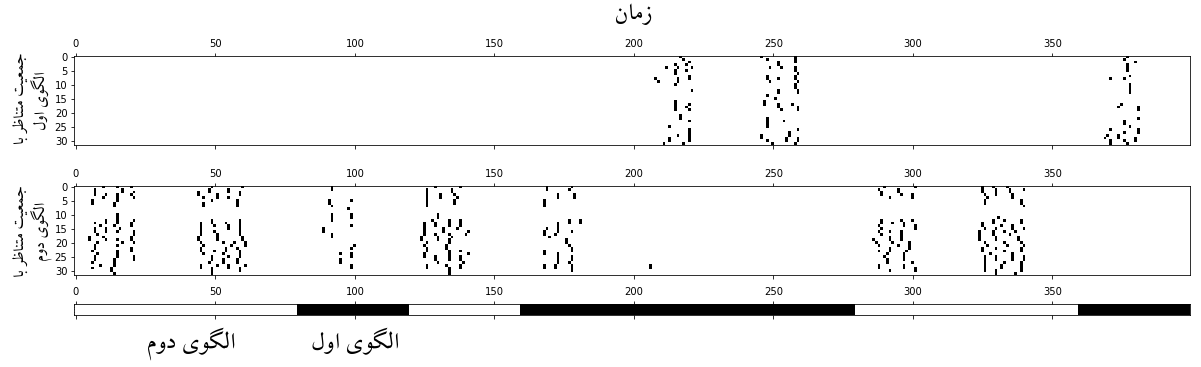
\includegraphics[width=1.0\linewidth]{c1-begining.png}
		\caption[NS]{
			\gls{rasterplot} مربوط به فعالیت نورون‌های جمعیت‌های لایه‌ی ۲/۳ ستون قشری در ۴۰۰ میلی‌ثانیه‌ی ابتدایی که در تصویر فوق، سطر اول فعالیت جمعیت نورونی متناظر با الگوی اول، سطر دوم جمعیت متناظر با الگوی دوم و نوار نمایش داده شده در سطر سوم نیز نمایش‌دهنده‌ی الگوی نشان داده شده در ورودی در آن زمان است که رنگ مشکی نشان‌‌دهنده‌ی نمایش الگوی اول در ورودی و رنگ سفید نشان‌دهنده‌ی نمایش الگوی دوم در ورودی است.
		}
		\label{fig:c1-begining} 
	\end{figure}
	
	با گذر زمان و پیشرفت فرآیند یادگیری هم‌بستگی بین ورودی و لایه‌ی ۲/۳ افزایش پیدا می‌کند؛ به طوری که فعالیت هر جمعیت از لایه‌ی ۲/۳ وابسته به نمایش الگوی متناظر با آن در جمعیت‌های ورودی می‌شود. یک نمونه فعالیت جمعیت‌های ستون قشری لایه‌ ۲/۳ در بازه‌ی زمانی  ۳۹۶۰۰ تا۴۰۰۰۰ میلی‌ثانیه (نمایش ۱۰ الگوی انتهایی) در تصویر \ref{fig:c1-final} نمایش داده شده‌است که افزایش هم‌بستگی در آن به وضوح قابل مشاهده است.
	
	\begin{figure}[]
		\centering
		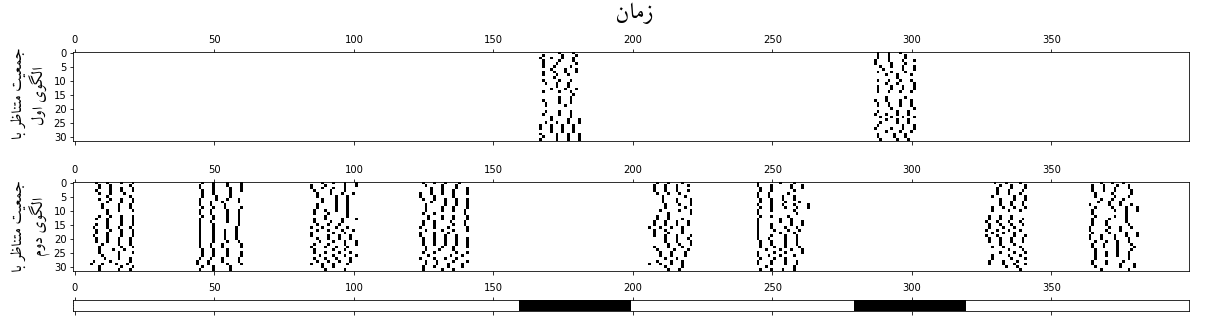
\includegraphics[width=1.0\linewidth]{c1-final.png}
		\caption[NS]{
			\gls{rasterplot} مربوط به فعالیت نورون‌های جمعیت‌های لایه‌ی ۲/۳ ستون قشری در بازه‌ی  ۳۹۶۰۰ و ۴۰۰۰۰ میلی‌ثانیه که در تصویر فوق، مشابه با تصویر \ref{fig:c1-begining} سطر اول فعالیت جمعیت نورونی متناظر با الگوی اول، سطر دوم جمعیت متناظر با الگوی دوم و نوار نمایش داده در سطر سوم نیز نمایش‌دهنده‌ی الگوی نشان داده شده در ورودی در آن زمان است که رنگ مشکی نشان‌‌دهنده‌ی نمایش الگوی اول در ورودی و رنگ سفید نشان‌دهنده‌ی نمایش الگوی دوم در ورودی است.
		}
		\label{fig:c1-final} 
	\end{figure}
	
	\subsection{نتایج آموزش ستون قشری سوم}
	
	همان‌طور که در بخش قبل‌ نیز به آن اشاره شد، پس از آموزش ستون‌های قشری متصل به ورودی، آن‌ها را به یک ستون قشری سوم متصل می‌کنیم و اتصالات بین آن‌ها را نیز برقرار می‌کنیم و مجدداً شبکه را آموزش می‌دهیم. در ابتدای این موضوع رفتار ستون قشری سوم بسیار نادقیق است ولی به‌مرور زمان رفتار نورون‌های حاضر در مدل به سمتی متمایل می‌شود که هم‌بستگی بین ورودی و رفتار جمعیت‌های لایه‌ی ۲/۳ ستون قشری سوم بسیار افزایش پیدا می‌کند. الگوی رفتاری جمعیت‌های لایه‌ی ۲/۳ ستون قشری سوم در ابتدا و انتهای بازه‌ی آموزش، به ترتیب در تصاویر ‌\ref{fig:c3-begining} و \ref{fig:c3-final} قابل مشاهده است.
	
	\begin{figure}[]
		\centering
		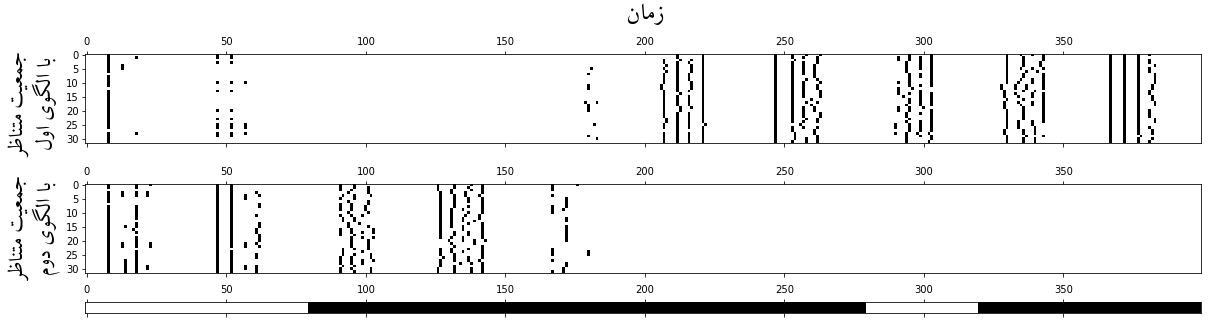
\includegraphics[width=1.0\linewidth]{c3-begining.png}
		\caption[NS]{
			فعالیت لایه‌ی ۲/۳ ستون قشری سوم در ۴۰۰ میلی‌ثانیه‌ی ابتدایی از آموزش ستون قشری سوم.
		}
		\label{fig:c3-begining} 
	\end{figure}

\begin{figure}[]
	\centering
	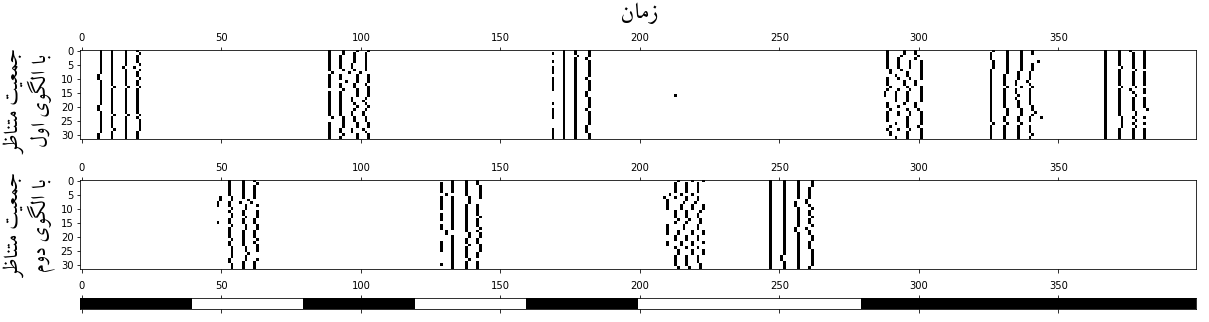
\includegraphics[width=1.0\linewidth]{c3-final.png}
	\caption[NS]{
	فعالیت لایه‌ی ۲/۳ ستون قشری سوم در ۴۰۰ میلی‌ثانیه‌ی انتهایی از آموزش ستون قشری سوم.
	}
	\label{fig:c3-final} 
\end{figure}
	
	\subsection{میزان پیشرفت یادگیری}
	
	در طول آموزش انتظار می‌رود وزن نورون‌های هر یک از اتصالات نورونی به یکی از مقادیر کمینه و بیشینه وزنش همگرا شود. بر همین اساس یک معیار همگرایی تعریف می‌شود که می‌توان با آن میزان پیشرفت یادگیری را اندازه‌گیری کرد. این معیار همگرایی برای سیناپس $i$ با وزن $w_i$ به صورت زیر تعریف می‌شود که همواره عددی بین صفر و یک می‌باشد:
	
	\begin{align}
		convergence_i = \frac{2 (w_i - w_{min})(w_{max} - w_i) }{ w_{max} - w_{min} }
		\label{eq:convergence_single}
	\end{align}

	به هر میزان که وزن به کمینه و بیشینه‌ی خود نزدیک‌تر باشد مقدار رابطه‌ی \ref{eq:convergence_single} نیز به صفر نزدیک‌تر می‌شود و بیشینه‌ی آن نیز در حالتی است که وزن نورون دقیقاً در نقطه‌ی میانگین کمینه و بیشینه قرار داشته‌باشد. همچنین از رابطه‌ی فوق می‌توان این معیار را برای یک مجموعه از سیناپس‌ها مثل $S$ به صورت زیر محاسبه کرد:
	
	\begin{align}
		convergence_{S} = \sum_{i \in S} \frac{convergence_i}{|S|} 
		\label{eq:convergence_pop}
	\end{align}
	
	تغییرات این معیار برای اتصالات مختلفی در طول یادگیری آن‌ها اندازه گرفته‌ شده‌است که نشان از همگرایی بسیار مناسب آن‌ها در بازه‌ی زمان دارد. برای نمونه نمودار تغییرات اتصالات مابین یکی از ستون‌های قشری متصل به ورودی و ستون قشری سوم در شکل \ref{fig:convergence} آورده شده‌است که همگرایی آن‌ها کاملاً در نمودار مشهود است.
	
	\begin{figure}[]
		\centering
		\subfigure[]{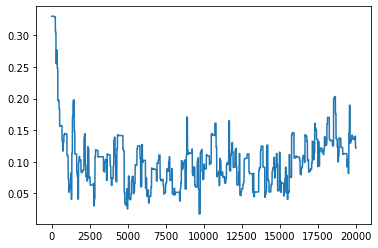
\includegraphics[width=0.45\textwidth]{conv1.png}} 
		\subfigure[]{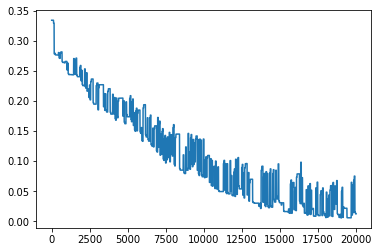
\includegraphics[width=0.45\textwidth]{conv2.png}} 
		\subfigure[]{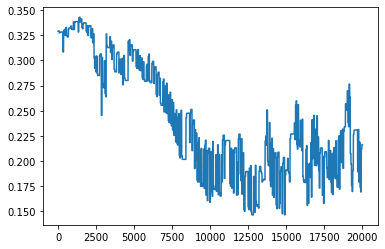
\includegraphics[width=0.45\textwidth]{conv3.png}}
		\subfigure[]{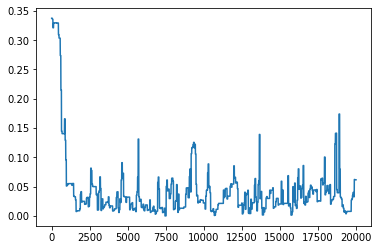
\includegraphics[width=0.45\textwidth]{conv4.png}}
		\caption{
			نمودار‌های مربوط به تغییرات معیار همگرایی وزن‌های اتصالات مابین جمعیت‌های لایه ۲/۳ یک ستون قشری متصل به ورودی و جمعیت‌های حاضر در لایه ۴ ستون قشری سوم.
			(آ) اتصالات بین دو جمعیت متناظر با الگوی اول.
			(ب) اتصالات بین جمعیت پیش‌سیناپسی متناظر با الگوی اول و جمعیت پس‌سیناپسی متناظر با الگوی دوم.
			(ج) اتصالات بین جمعیت پیش‌سیناپسی متناظر با الگوی دوم و جمعیت پس‌سیناپسی متناظر با الگوی اول. 
			(د) اتصالات بین دو جمعیت متناظر با الگوی دوم.
		}
		\label{fig:convergence}
	\end{figure}
	
	\subsection{بررسی وجود انقیاد در مدل}
	
	در مدل ارائه‌شده، فعالیت هم‌زمان دو ورودی مجزا، که هر یک بیانگر یک \gls{sensory-input} هستند،  پس از آموزش موجب فعالیت در ستون قشری سوم می‌شود که بیان‌گر یک مفهوم انتزاعی از چیزی است که دو ورودی حسی متعلق به آن هستند. در صورت رخدادن انقیاد در مدل باید فعالیت حتی یکی از ورودی‌ها نیز باعث فعال‌شدن شبکه‌های عصبی متناظر با مفهوم کلی مورد نظر شود که به عبارت دیگر، تنها در صورت فعالیت یکی از ورودی‌ها باید شاهد رفتار درست لایه‌ی ۲/۳ ستون قشری سوم باشیم.
	برای بررسی این مورد یکی از جمعیت‌های ورودی را مشابه با زمان آموزش فعال کرده و جمعیت دیگر را بدون هیچ الگویی و تنها با مجموعه‌ای از فعالیت‌های تصادفی تعریف می‌کنیم و انتظار داریم در ستون قشری سوم فعالیت مورد نظر را مشاهده کنیم. \gls{rasterplot} مربوط به جمعیت‌های ورودی و جمعیت‌های لایه ۲/۳ ستون قشری سوم در یک بازه‌ی زمانی ۴۰۰ میلی‌ثانیه‌ای در تصویر \ref{fig:binding-c1-c3} آورده شده‌ و کاملاً مشهود است که با وجود این‌که در جمعیت ورودی دوم، الگویی نمایش داده نشده و تنها مجموعه ای از فعالیت‌های تصادفی اتفاق افتاده، هر دو جمعیت ستون قشری سوم فعالیت صحیح و مورد انتظاری دارند که در نتیجه انقیاد در این شبکه شکل گرفته است. هم‌چنین این موضوع به صورت برعکس،یعنی به صورتی که جمعیت ورودی فعال در تصویر \ref{fig:binding-c1-c3} غیر‌فعال باشد و جمعیت دیگر فعال باشد نیز مورد بررسی قرار گرفته (تصویر \ref{fig:binding-c2-c3}) و صادق بودن این موضوع در آن حالت نیز مشخص شده‌ است.
	
	\begin{figure}[]
		\centering
		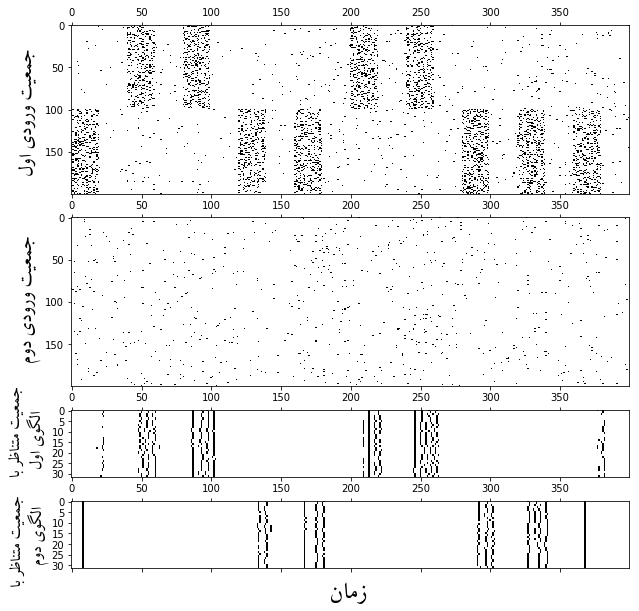
\includegraphics[width=1.0\linewidth]{binding-c1-c3.png}
		\caption[NS]{
			تصویر مربوط به بررسی وجود انقیاد در زمان نمایش الگو توسط جمعیت ورودی اول. در تصویر فوق سطر اول فعالیت جمعیت ورودی اول، سطر دوم جمعیت ورودی دوم و سطر سوم و چهارم نیز نشان‌دهنده‌ی فعالیت جمعیت‌های لایه‌ی ۲/۳ ستون قشری سوم هستند.
		}
		\label{fig:binding-c1-c3} 
	\end{figure}

\begin{figure}[H]
	\centering
	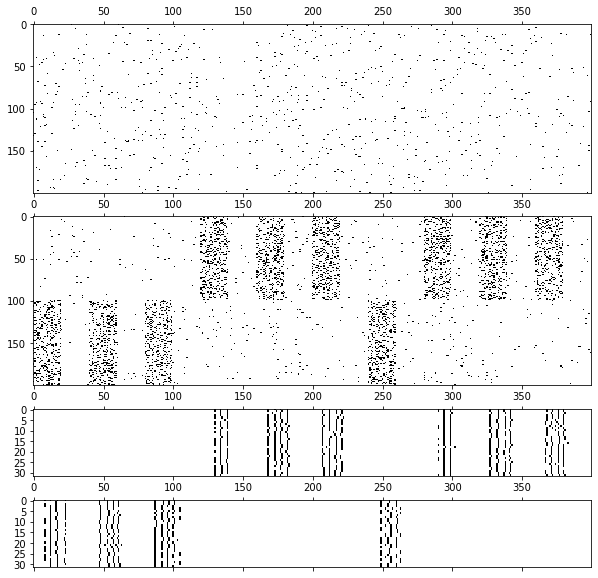
\includegraphics[width=1.0\linewidth]{binding-c2-c3.png}
	\caption[NS]{
		تصویر مربوط به بررسی وجود انقیاد در زمان نمایش الگو توسط جمعیت ورودی دوم. مشابه با تصویر \ref{fig:binding-c1-c3}، در این تصویر نیز سطر اول فعالیت جمعیت ورودی اول، سطر دوم جمعیت ورودی دوم و سطر سوم و چهارم نیز نشان‌دهنده‌ی فعالیت جمعیت‌های لایه‌ی ۲/۳ ستون قشری سوم هستند.
	}
	\label{fig:binding-c2-c3} 
\end{figure}

	
	\section{مقایسه‌ی مدل ارائه‌شده با مدل‌های پیشین}
	چنان‌چه پیش از این نیز اشاره شد، در مدل‌های پیشین از روش‌های گوناگونی برای مدل‌سازی انقیاد استفاده شده‌است. اما، حتی در نزدیک‌ترین مدل ارائه‌شده به ساختار‌های زیستی نیز فاصله‌ی قابل توجهی با واقعیت وجود داشت. در این پژوهش تلاش شده تا مدل ارائه‌شده از تمام جنبه‌ها یک مدل بسیار نزدیک به ساختار مغز باشد. چنانچه برای مدل‌سازی نورون‌ها از شبکه‌های عصبی ضربه‌ای استفاده شده که نزدیک‌ترین مدل‌های نورونی به نورون‌های زیستی هستند و برای توپولوژی آن‌ها نیز تلاش شده از یک الگوی ارتباطی بسیار مشابه با ستون‌های قشری حاضر در نوقشر الگوبرداری شود تا از هر جهت یک مدل نزدیک به ساختار زیستی باشد.
	
	این در حالی است که در تحقیقاتی که پیش از این صورت گرفته است، در بسیاری از موارد ساختار ارتباطی و نورون‌ها هیچ شباهتی به مدل‌های زیستی ندارند. مواردی همچون استفاده از شبکه‌های عصبی رمزگذار-رمزگشای مولد که یک نمونه از مواردی است که از ساختار زیستی فاصله دارند.
	
	در این دسته از مدل‌سازی‌ها که هدف آن‌ها ارائه‌ی یک رویکرد و ساختار محاسباتی برای حل مسئله‌ی انقیاد است و در حال حاضر برای مسائلی همچون دسته‌بندی یا رگرسیون از آن‌ها استفاده نمی‌شود، برای مقایسه معیار عددی مشخصی نمی‌توان تعریف کرد ولی با توجه به هدف نهایی، شکل‌دادن انقیاد و علم به رخدادن آن در مغز و اهمیت آن در ادراک مدل‌های مبتنی بر زیست، این مدل‌سازی‌ها در صورت نشان دادن عملکرد مناسب بسیار ارزشمند هستند.
	
	\section{نتیجه‌گیری}
	در این پژوهش نشان داده‌شد که ستون‌های قشری توانایی پردازش اطلاعات و  شکل‌دادن انقیاد را دارند که یک عملکرد شناختی بسیار مهم و پیچیده در پستانداران است و این امکان وجود دارد که مشابه با انقیاد، ستون‌های قشری توانایی تشکیل بسیاری دیگر از عملکرد‌های شناختی را داشته باشند. این یک گام به سوی ساختن عامل‌هایی با هوشمندی مشابه با موجودات زنده است.
	
	همچنین این ویژگی ستون‌های قشری که ساختار و الگوی ارتباطی یکسانی دارند، باعث می‌شود تا بتوان از آن‌ها به سادگی به عنوان بلوک‌هایی تکرار‌شونده در شبکه‌های عصبی استفاده کرد و شبکه‌هایی ساخت که با از کنار هم قرارگرفتن مجموعه‌ای از ستون‌های قشری، قادر به مدل‌سازی عملکرد‌های پیچیده‌ای هستند.
	
	\section{فعالیت‌های آینده}
	در این پژوهش هر لایه از ستون‌های قشری به دو دسته تقسیم شده‌بود تا فرایند یادگیری و تفکیک فعالیت نورون‌های مقید‌شده به هر الگوی ورودی مشخص‌تر باشد. از جمله کار‌هایی که می‌توان در ادامه‌ی این پژوهش انجام داد، این است که تعداد جمعیت‌‌های داخل هر لایه افزایش یابد تا بتوان تفکیک را بین بیش از دو الگو نیز با استفاده از ستون‌های قشری انجام داد. همچنین می‌توان به جای در نظرگرفتن تعداد مشخصی جمعیت، هر لایه را یک جمعیت یکپارچه در نظر گرفت و انتظار داشت در طول آموزش، هر نورون به‌مرور زمان به یکی از الگو‌های ورودی مقید شود که  مدلی بسیار نزدیک‌تر به ساختار زیستی مغز و ستون‌های قشری حاضر در مغز است. همچنین یکی دیگر از مطالعاتی که می‌توان در راستای این پژوهش انجام داد، استفاده از \gls{dataset}‌های حقیقی همچون MNIST\LTRfootnote{Modified National Institute of Standards and Technology database}
در عوض استفاده‌کردن از الگوی تصادفی در ورودی است. هم‌چنین می‌توان در یکی از ورودی‌ها، داده‌ای از یک جنس و در یکی دیگر از ورودی‌ها، داده‌ای از جنس دیگر استفاده کرد. برای نمونه، در یکی از تصویر و در دیگری از صوت متناظر با آن تصویر استفاده کرد و انتظار داشت تا یک مفهوم حاصل از انقیاد صوت و تصویر شکل بگیرد.
	
	
	
	%#######################################################
	%#######################################################
	%#######################################################
	%#######################################################
	
	
	
	%Glossaries-----------------------------------
	
	\printglossary[title=واژه‌نامه فارسی به انگلیسی, toctitle=واژه‌نامه فارسی به انگلیسی]
	
	%References-----------------------------------
	
	%\begin{thebibliography}{MM}
	\begin{latin}
		\bibliographystyle{abbrv}
		\renewcommand{\bibname}{\rl{{مراجع}\hfill}}
		%	\addcontentsline{toc}{chapter}{کتاب‌نامه}
		\bibliography{references}
	\end{latin}
	%\end{thebibliography}
	
	%Abstract En----------------------------------
	\linespread{1}
	\begin{latin}
		\begin{abstract}
			Binding problem is one of the important problems in neuroscience, cognitive sciences and philosophy of mind. It's about how a living organism's understanding is integrated from partial concepts formed in the brain. The importance of this problem is in understanding of human cognitive functions, which itself is the part of steps required to designing systems that are capable of processing human-like cognitive functions. Researches show the very strong role of cortical columns, which are structures in the neocortex, in the cognitive functions of living organisms. In this research, we tried to simulate the formation of binding in the brain by modeling the cortical columns and the relationships between them using spiking neural networks. Finally, the tests and investigations carried out on the designed model show the formation of binding in the proposed model. This indicates that probably the cortical columns, as defined structures that can be easily replicated in modeling, are potentially suitable structures to be used in modeling and increase the possibility of forming cognitive processes in the model.
			
			\section*{}
			\textbf{Keywords:}\quad Cortical Column, Binding Problem, Spiking Neural Network, Modeling.
		\end{abstract}
		\newpage
		
		%Title page En -------------------------------
		\begin{figure}
			\centering
			
\includegraphics[height=2.5cm]{ut.png}
		\end{figure}
		\begin{center}
			
			College of Science\\
			School of Mathematics, Statistics, and Computer Science
		\end{center}
		
		\begin{center}
			%%%%%%%%%%%%%
		\end{center}
		
		\begin{center}
			\huge{Modeling the Mechanisms of Binding Problem in Spiking Neural Networks}
		\end{center}
		
		\begin{center}
			%%%
		\end{center}
		
		\begin{center}
			\textbf{
				Amir Aslan Aslani
				\\[30pt]
			}
		\end{center}
		
		
		\begin{center}
			Supervisors
		\end{center}
		\begin{center}
			\textbf{
				Mohammad Ganjtabesh
				\\[5pt]
				Abbas Nouzari-Dalini
			}
		\end{center}
		
		
		\vspace{3cm}
		\begin{center}
			A thesis submitted to Graduate Studies Office\\
			in partial fulfillment of the requirements for the degree of \\
			Master of Science in\\
			Computer Science
		\end{center}
		
		\begin{center}
			February 2022
		\end{center}
		
		%\pagestyle{empty}
		%\pagenumbering{}
		
	\end{latin}
	
\end{document}
%####################################################################
%########### END DOCUMENT ###########################################
%####################################################################